 %%%%%%%%%%%%%%%%%%%%%%%%%%%%%%%%%%%%%%%%%%%%%%%%%%%%%%%%%%%%%%%%%%%%%
% LaTeX Template: Project Titlepage Modified (v 0.1) by rcx
%
% Original Source: http://www.howtotex.com
% Date: February 2014
% 
% This is a title page template which be used for articles & reports.
% 
% This is the modified version of the original Latex template from
% aforementioned website.
% 
%%%%%%%%%%%%%%%%%%%%%%%%%%%%%%%%%%%%%%%%%%%%%%%%%%%%%%%%%%%%%%%%%%%%%%

\documentclass[12pt]{article}

\usepackage{ctex}
\usepackage[a4paper]{geometry}
\usepackage[myheadings]{fullpage}
\usepackage{adjustbox}
\usepackage{fancyhdr}
\usepackage{lastpage}
\usepackage{graphicx, wrapfig, subcaption, setspace, booktabs}
\usepackage{epsfig}
\usepackage{epstopdf}
\usepackage[T1]{fontenc}
\usepackage[font=small, labelfont=bf]{caption}
\usepackage{fourier}
\usepackage[protrusion=true, expansion=true]{microtype}
\usepackage[english]{babel}
\usepackage{sectsty}
\usepackage{url, lipsum}
\usepackage{tgbonum}
\usepackage{hyperref}
\usepackage{xcolor}
\usepackage{listings}
\usepackage{fontspec}
\newfontfamily\cn{Courier New}
\hypersetup{colorlinks=true, linkcolor=black}

\newcommand{\HRule}[1]{\rule{\linewidth}{#1}}
\onehalfspacing
\setcounter{tocdepth}{5}
\setcounter{secnumdepth}{5}

\lstset{
	xleftmargin=2em,
	numbers=left,
	framexleftmargin=10mm,
	frame=none,
	basicstyle=\cn,
	keywordstyle=\bf\cn,
	identifierstyle=\cn,
	numberstyle=\cn,
	commentstyle=\cn,
	stringstyle=\cn,
	showstringspaces=false,
	breaklines=true, 
	breakautoindent=true,
	breakindent=2em, 
	tabsize=4,
}

%-------------------------------------------------------------------------------
% HEADER & FOOTER
%-------------------------------------------------------------------------------
%\pagestyle{fancy}
%\fancyhf{}
%\setlength\headheight{15pt}
%\fancyhead[L]{Student ID: 1034511}
%\fancyhead[R]{Anglia Ruskin University}
%\fancyfoot[R]{Page \thepage\ of \pageref{LastPage}}
%-------------------------------------------------------------------------------
% TITLE PAGE
%-------------------------------------------------------------------------------

\begin{document}
{\fontfamily{cmr}\selectfont
\title{ \normalsize \textsc{}
		\\ [2.0cm]
		\HRule{0.5pt} \\
		\LARGE \textbf{\uppercase{计算机组成原理——流水硬连线控制器的设计}
		\HRule{2pt} \\ [0.5cm]
		\normalsize \today \vspace*{5\baselineskip}}
		}

\date{}

\author{
		房庆凯\ 2017211131 \\
		陈政瑞\ 2017211130}

\maketitle
\clearpage
\tableofcontents

\clearpage

%-------------------------------------------------------------------------------
% Section title formatting
\sectionfont{\scshape}
%-------------------------------------------------------------------------------

%-------------------------------------------------------------------------------
% BODY
%-------------------------------------------------------------------------------

\section{设计目的}
    \begin{itemize}
        \item 融会贯通计算机组成与体系结构课程各章教学内容,通过知识的综合运用,加深对 CPU 各模块工作原理及相互联系的认识。
        \item 掌握流水硬连线控制器的设计方法。
        \item 学习运用当代的 EDA 设计工具,掌握用 EDA 设计大规模复杂逻辑电路的方法。
        \item 培养科学研究能力,取得设计和调试的实践经验。
    \end{itemize}
    
\section{实验设备}
    \begin{itemize}
        \item TEC-8 实验系统            1 台
        \item 计算机                    1 台
    \end{itemize}   
    
\section{硬件环境}
    本次设计在 TEC-8 模型机上完成。
    \subsection{模型计算机时序信号}
        TEC-8 模型计算机主时钟 $MF$ 的频率为 $1MHz$,执行一条微指令需要 $3$ 个节拍脉冲 $T1$、$T2$、$T3$。TEC-8 模型计算机时序采用不定长机器周期,绝大多数指令采用 $2$ 个机器周期 $W1$、$W2$,少数指令采用一个机器周期 $W1$ 或者 $3$ 个机器周期 $W1$、$W2$、$W3$。
        
        $3$ 个机器周期的时序图如 Figure\ref{fig:4-1-1} 所示。
        
        \begin{figure}[!ht]
            \centering
            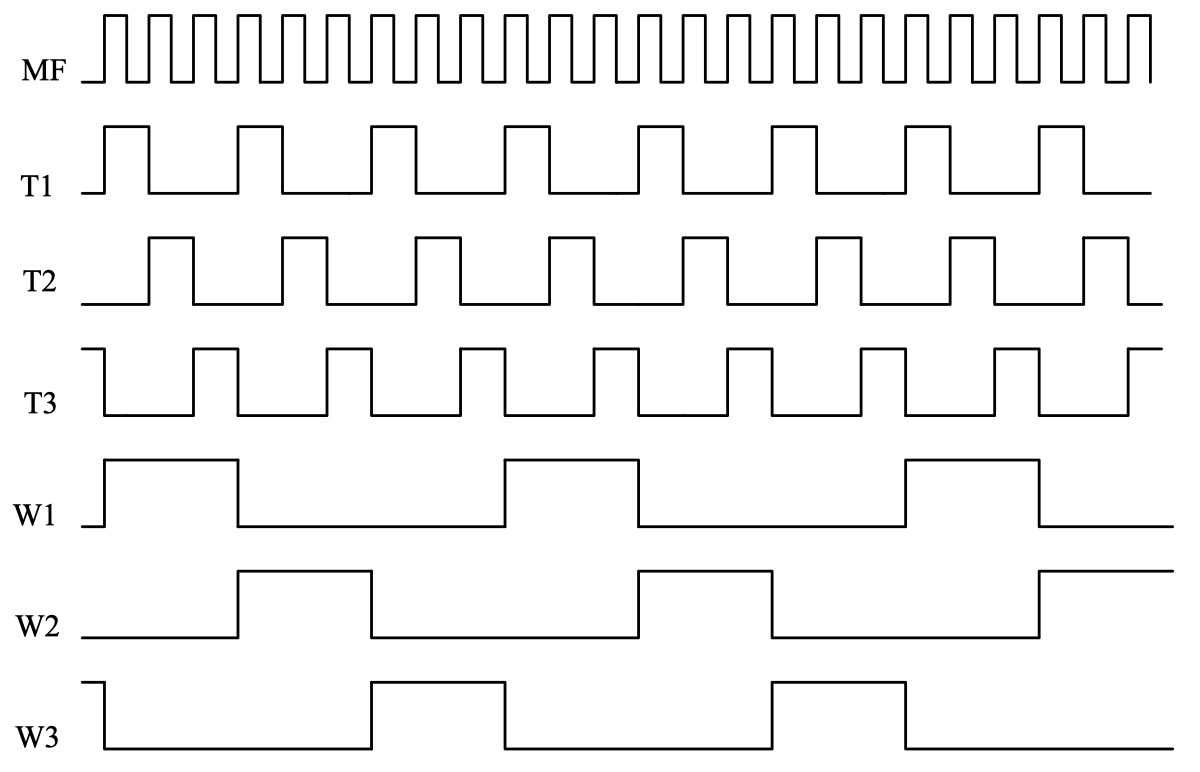
\includegraphics[width=1.0\textwidth]{时序图.png}
            \caption{TEC-8 模型计算机时序图}
            \label{fig:4-1-1}
        \end{figure}
        
    \subsection{组成模块 \& 数据通路}
        如 Figure\ref{fig:4-1-2} 所示。
        
        \begin{figure}[!ht]
            \centering
            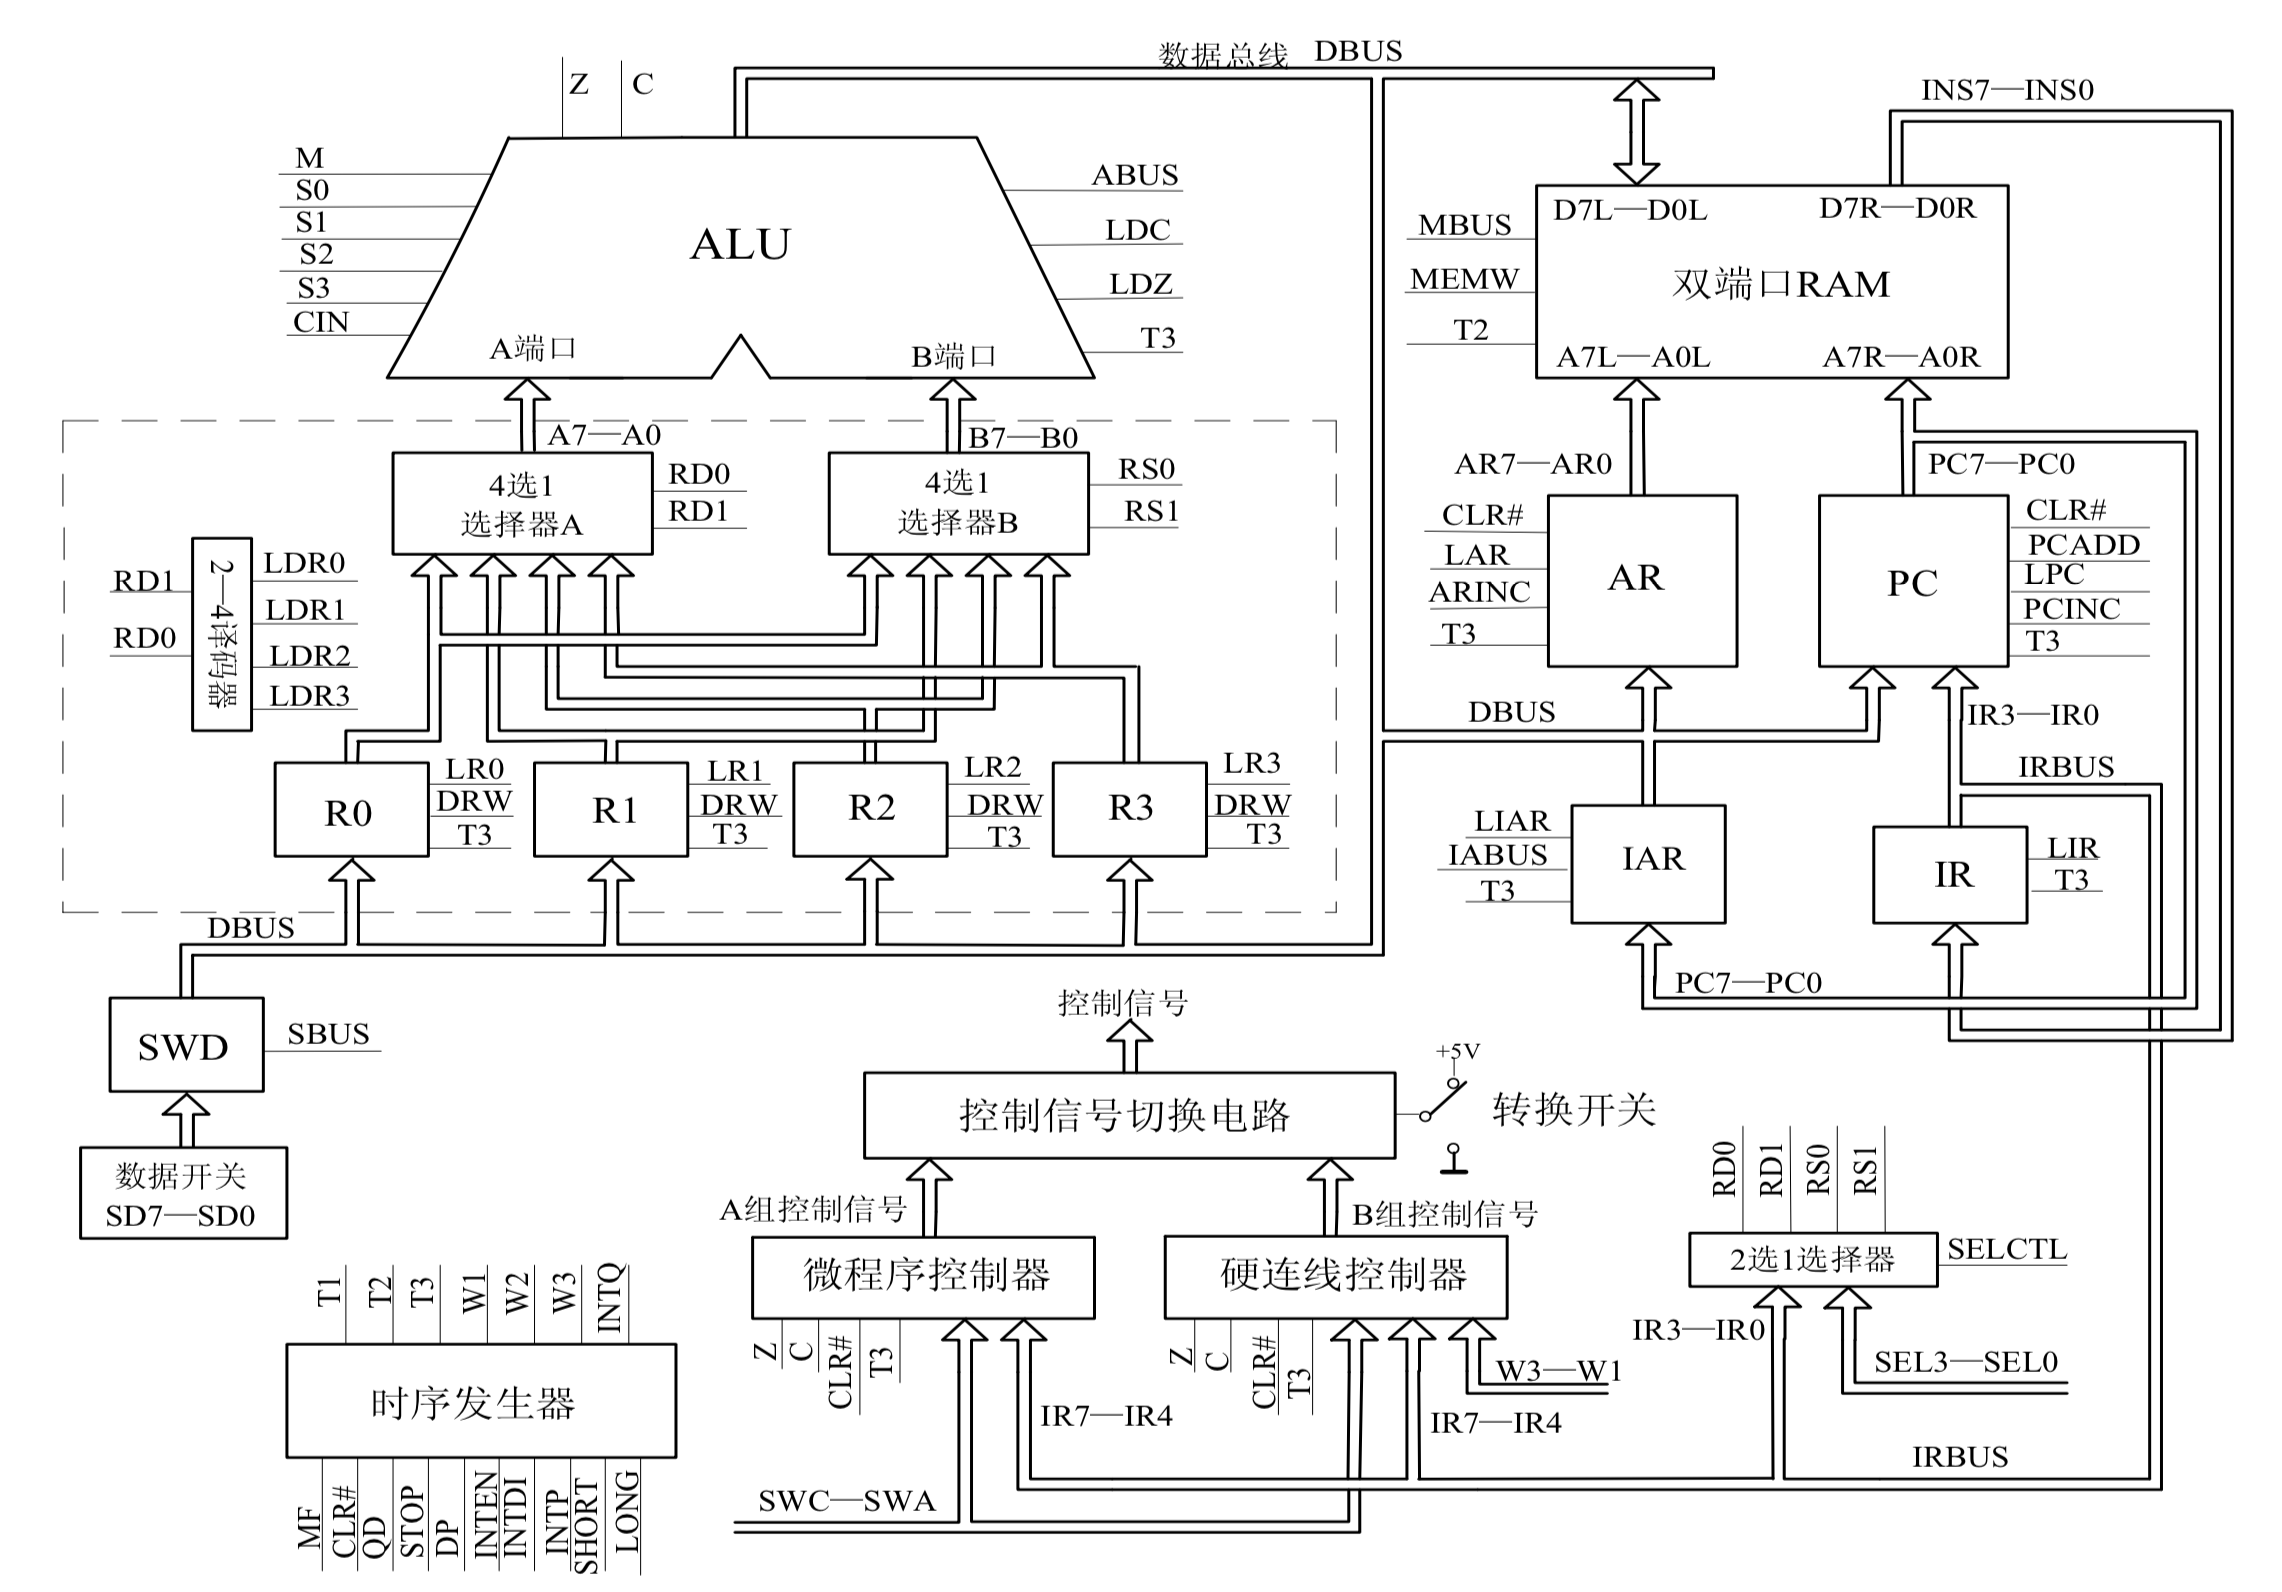
\includegraphics[width=1.0\textwidth]{数据通路.png}
            \caption{TEC-8 模型计算机框图}
            \label{fig:4-1-2}
        \end{figure}
    
    \subsection{EPM 7128 器件的引脚}
        TEC-8 实验系统中的硬连线控制器是用 $1$ 片 EPM7128 器件构成的。硬连线控制器和数据通路之间在印制电路板上已经用印制导线进行了连接。因此硬连线控制器所需的信号的输出、输入信号的引脚号必须符合 Figure\ref{fig:4-1-3} 中的规定。
        
        \begin{figure}[!ht]
        	\centering
        	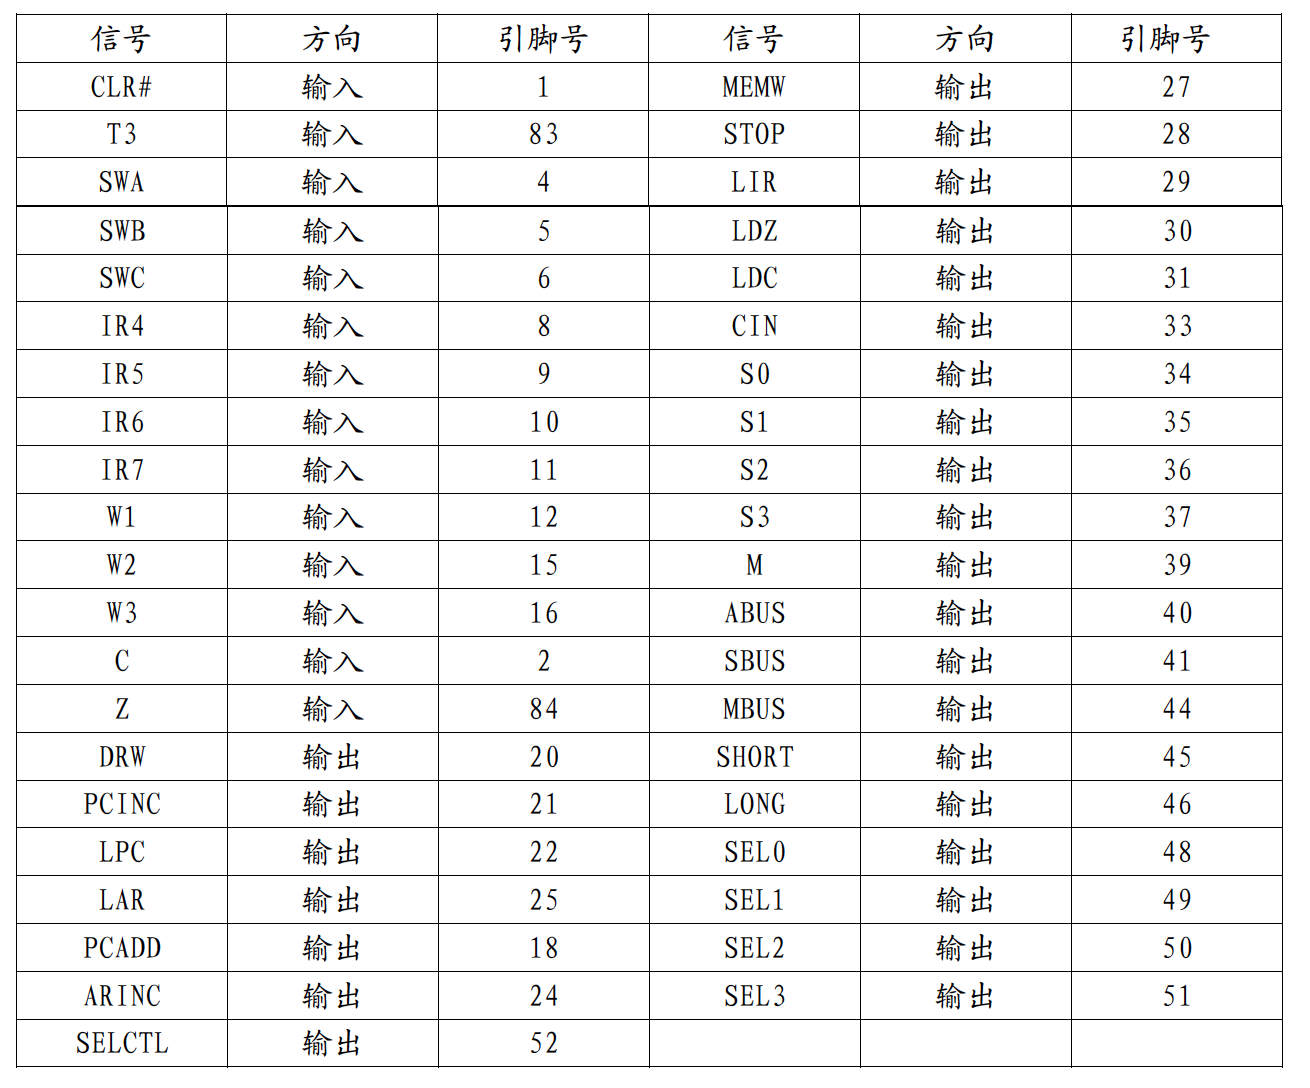
\includegraphics[width=1.0\textwidth]{引脚.png}
        	\caption{EPM 7128 器件的引脚}
        	\centering
        	\label{fig:4-1-3}
        \end{figure}
    
\section{设计与调试任务}
    \begin{itemize}
        \item 设计一个流水硬连线控制器,和 TEC-8 模型计算机的数据通路结合在一起,构成一个完整的 CPU,该 CPU 要求:
        \begin{itemize}
            \item 能够完成控制台操作:启动程序运行、读存储器、写存储器、读寄存器和写寄存器。
            \item 能够执行Figure\ref{fig:3} 中的指令(扩展了 $3$ 条指令),完成规定的指令功能。
        \end{itemize}
        \item 在 Quartus \uppercase\expandafter{\romannumeral2} 下对硬连线控制器对设计方案进行编程和编译
        \item 将编译后的流水硬连线控制器下载到 TEC-8 实验台上的 ISP 器件 EPM7128 中去,使 EPM7128 成为一个流水硬连线控制器。
        \item 根据指令系统,编写检测硬连线控制器正确性的测试程序,并用测试程序对硬布线控制器在单拍方式下进行调试,直到成功。
        \item 在调试成功的基础上,整理出设计文件。
    \end{itemize}
    
    \begin{figure}[!ht]
    	\centering
    	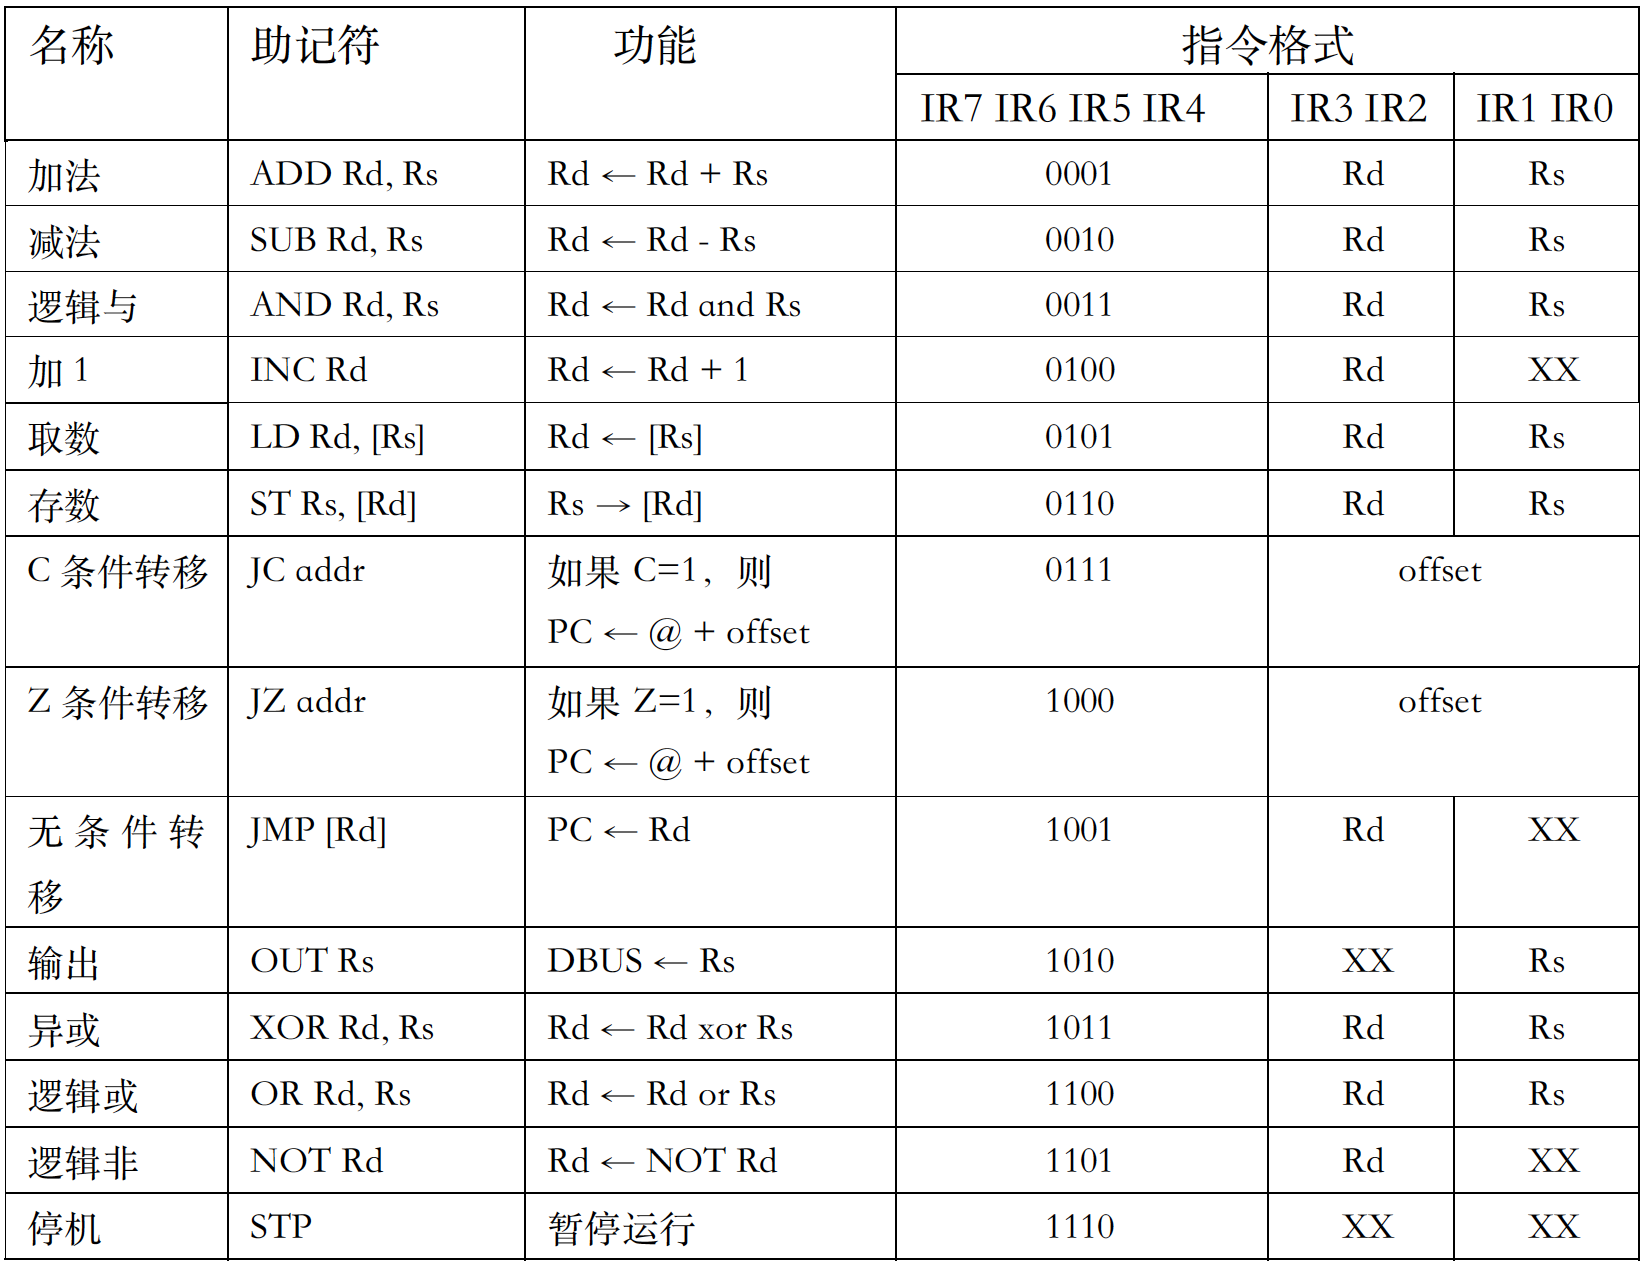
\includegraphics[width=1.0\textwidth]{指令系统.png}
    	\caption{CPU指令系统}
    	\centering
    	\label{fig:3}
    \end{figure}

\section{实验原理}
    \subsection{硬连线控制器}
        \subsubsection{基本原理}
            硬连线控制器的基本原理,每个微操作控制信号 $S$ 是一系列输入量的逻辑函数,即用组合逻辑来实现,$S=f(I_m,M_i,T_k,B_j)$,其中 $I_m$ 是机器指令操作码译码器的输出信号,$M_i$ 是节拍电位信号,$T_k$ 是节拍脉冲信号,$B_j$ 是状态条件信号。
            
            在 TEC-8 实验系统中,节拍脉冲信号 $T_k(T1\sim T3)$ 已经直接输送给数据通路。因为机器指令系统比较简单,省去操作码译码器,4 位指令操作码 $IR4\sim IR7$ 直接成为 $I_m$ 的一部分;由于 TEC-8 实验系统有控制台操作,控制台操作可以看作一些特殊的功能复杂的指令,因此 $SWC$、$SWB$、$SWA$ 可以看作是 $I_m$ 的另一部分。$M_i$ 是时序发生器产生的节拍信号 $W1\sim W3$;$B_j$ 包括 ALU 产生的进位信号 $C$、结果为 $0$ 信号 $Z$ 等等。
            
        \subsubsection{执行一条机器指令的节拍电位数}
            在 TEC-8 实验系统中,采用了可变节拍电位数来执行一条机器指令。大部分指令的执 行需要 $2$ 个节拍电位 $W1$、$W2$。
        
            对于一些控制台操作,需要 $4$ 个节拍电位才能完成规定的功能。为了满足这种情况, 可以将控制台操作化成两条机器指令的节拍。为了区分写寄存器操作的 $2$ 个不同阶段,可以用某些特殊的寄存器标志标。例如建立一个 $ST0$ 标志,当 $ST0=0$ 时,表示该控制台操作的第 $1$ 个 $W1$、$W2$;当 $ST0=1$ 时,表示该控制台操作的第 $2$ 个 $W1$、$W2$。
    
            为了适应更为广泛的情况,TEC-8 的时序信号发生器允许只产生一个节拍电位 $W1$。当 $1$ 条指令或者一个控制台在 $W1$ 时,只要产生信号 $SHORT$,该信号送往时序信号发生器,则时序信号发生器在 $W1$ 后不产生节拍电位 $W2$,下一个节拍仍是 $W1$。信号 $SHORT$ 只对紧跟其后的第一个节拍电位的产生起作用。
            
        \subsubsection{硬连线控制器 VS 微程序控制器}
            硬连线控制器通过每条指令读取时执行相应的硬件管脚信号来实现一条指令对应多个微操作,操作多个硬件来实现一条指令的复杂功能。而微程序控制器则通过将一条指令所需要的微操作制作成微指令存储到微指令存储器当中,当读取一条指令的时候,通过将微指令存储器中的微指令读出到微指令寄存器中,再依次执行,可以实现一条指令的执行。
            
            硬连线控制器更加高效,因为我们通过逻辑操作控制不同微操作的执行,而微程序控制器则需要从微指令存储器中读取,效率较低。同样的,硬连线控制器因为需要实现复杂的逻辑操作,实现难度较高。
            
    \subsection{流水}
        \subsubsection{基本原理}
            利用流水可以提高指令执行的速度,其关键在于将两条或者多条指令在时间上重叠起来
            ,在空间上分时共享不同的部件。比如将前一条指令的执行和当前指令的取指放到同一个节拍点位中执行。
            
            下面 Figure\ref{fig:4-3-1} 是流水硬连线的时空图,在这里我们将流水与硬连线结合起来,对于$SHORT$类型的指令,当时序信号发生器产生节拍电位$W1$时,我们不仅执行当前指令,而且通过$LIR$将下一条指令读取到指令寄存器当中,并且$PCINC$将$PC$加$1$,便于读取后面的指令。对于$LD, ST$等需要两个节拍的指令,我们在第二个节拍电位$W2$的时候添加了读取下一条指令的$LIR, PCINC$操作,实现流水。
            
            \begin{figure}
                \centering
                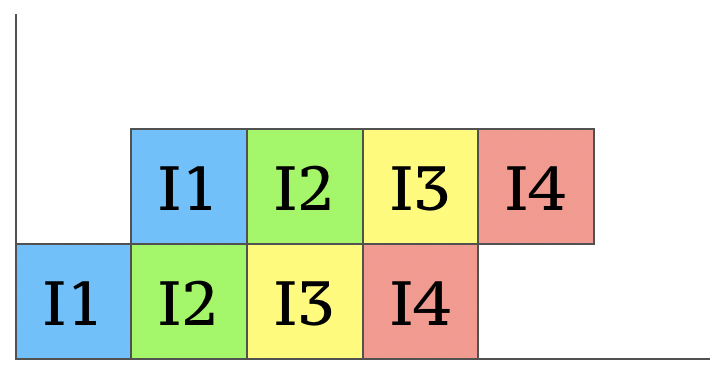
\includegraphics[width=1.0\textwidth]{流水.png}
                \caption{流水硬连线时空图}
                \label{fig:4-3-1}
            \end{figure}
            
        \subsubsection{流水 VS 非流水}
            流水可以大幅提高我们的执行效率。拿非流水的硬连线控制器来说,当没有流水,执行每一条指令时的第一个节拍电位都是用来执行$LIR, PCINC$读取指令的。下面 Figure\ref{fig:4-3-2} 是非流水硬连线的流水时空图,在这里可以跟上面的流水硬连线时空图进行对比,可以看到当同样运行了两条指令之后,流水硬连线的执行时间是非流水的$\frac{3}{4}$。而且,流水层级越高,执行时间越长,流水的效率就越高。
            
            \begin{figure}
                \centering
                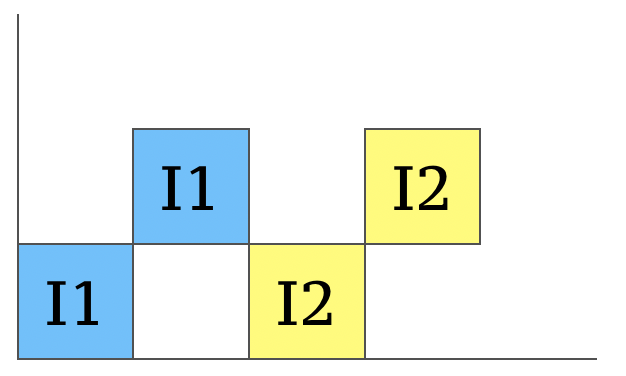
\includegraphics[width=1.0\textwidth]{非流水.png}
                \caption{非流水硬连线时空图}
                \label{fig:4-3-2}
            \end{figure}
    
\section{题目分析与设计详解}
    \subsection{基础部分}
        冯·诺伊曼型计算机的 CPU,其工作可以分为 $5$ 个阶段:取指令、指令译码、执行指令、访存取数、结果写回。
        
        在这里,由于指令系统比较简单,我们省去了指令译码这一步。访存取数、结果写回也可以看成是执行指令的一部分。因此我们可以将 CPU 的工作简单分为取指令、执行指令两个阶段。
        
        执行程序之前,我们需要把写好的程序(指令序列)写入存储器里面,取指令时,我们需要从存储器里读出下一条指令。执行指令时,我们又要根据指令内容对寄存器进行读、写操作。综上,我们需要实现读寄存器、写寄存器、读存储器、写存储器、取指。在程序中执行哪个操作是通过 $SWC$、$SWB$、$SWA$ 来决定的。下面我们来逐条分析如何实现。
        
        \subsubsection{读寄存器}
            读寄存器需要 $2$ 个节拍电位,$W1$ 时我们将 $SEL3$、$SEL2$ 设为 $00$,将 $SEL1$、$SEL0$ 设为 $01$,这时寄存器 $R0$ 的值会送往 ALU 的 A 端口,$R1$ 的值会送往 ALU 的 B 端口。我们可以通过指示灯 $A7\sim A0$、$B7\sim B0$ 来观察到这两个值。同理,在 $W2$ 节拍我们可以读出 $R2$、$R3$ 寄存器的值。
        
        \subsubsection{写寄存器}
            首先这里我们需要先打开 $SBUS$ 和 $DRW$,$SBUS=1$ 允许我们将数据开关的值送到数据总线上,$DRW=1$ 时在 $T3$ 上升沿对 $RD1$、$RD0$,即 $SEL3$、$SEL2$ 选中的寄存器进行写操作,将数据总线上的值写入选定的寄存器。
            
            写寄存器需要 $4$ 个节拍电位,我们将其化成两条机器指令的节拍,通过 $ST0$ 来区分。第一个 $W1$ 时我们将 $SEL3$、$SEL2$ 设为 $00$,将 $SEL1$、$SEL0$ 设为 $11$,表示向 $R0$ 寄存器里写入值。接下来 $W2$ 我们将 $SEL3$、$SEL2$ 设为 $01$,将 $SEL1$、$SEL0$ 设为 $00$,表示向 $R1$ 写入值,并读取 $R0$ 的值。之后也类似,每次 $SEL3$、$SEL2$ 指定当前写入的寄存器,$SEL1$、$SEL0$ 指定上次写入的寄存器,这样每次可以在 ALU 的 B 端口,即 $B7\sim B0$ 指示灯检查上次写入的值是否正确。注意到在第一个 $W2$ 节拍时,将 $SST0$ 标志置为 $1$,然后在 $T3$ 的下降沿就会将 $ST0$ 从 $0$ 变为 $1$,表示我们进入到第二个 $W1$、$W2$。
        
        \subsubsection{读存储器}
            读存储器可以分为两个步骤:指定首地址,依次读取存储单元。我们可以通过 $ST0$ 来区分这两个步骤。
            
            开始时 $ST0=0$,我们打开 $SBUS$,打开 $LAR$,将数据开关的值送入地址寄存器 $AR$,这样就实现了指定首地址。同时我们将 $SST0$ 置为 $1$,表示我们即将进入 $ST0=1$,即读存储器的阶段。
            
            读存储器时,我们将 $MBUS$ 打开,就可以把当前指定存储单元的值读到数据总线上,在 $D7\sim D0$ 指示灯观察。然后我们执行 $ARINC$ 来将 $AR$ 加一,在下一个节拍中读取下一个存储单元的值。
        
        \subsubsection{写存储器}
            写存储器也可以分为两个步骤:指定首地址,依次写入存储单元。我们可以通过 $ST0$ 来区分这两个步骤。
           
            开始时 $ST0=0$,我们打开 $SBUS$,打开 $LAR$,将数据开关的值送入地址寄存器 $AR$,这样就实现了指定首地址。同时我们将 $SST0$ 置为 $1$,表示我们即将进入 $ST0=1$,即写存储器的阶段。
            
            写存储器时,我们将 $MEMW$ 打开,就可以把当前数据总线上的值存入指定存储单元。然后我们执行 $ARINC$ 来将 $AR$ 加一,在下一个节拍中向下一个存储单元写入值。
            
        \subsubsection{执行程序}
            有了以上四个操作的支持,我们就可以把程序存到存储器里,设置寄存器和存储器的初始值,然后开始执行了。
            
            在按下复位按钮 $CLR$ 后,指令寄存器 $IR$ 被复位为 $00H$,因此当我们进入执行程序阶段时,第一条执行的指令永远是 $NOP$,即一条空指令。然后我们通过 $LIR$、$PCINC$ 来取出第一条指令,开始执行我们的程序。之后在每个机器指令结束时取出下一条指令,也就是上文我们提到的流水,之后程序就可以一直执行下去了。
            
        \subsubsection{机器指令周期流程图设计}
            我们使用流程图来设计硬连线控制器,硬连线控制器的控制信号以节拍电位(CPU 周期)为时间单位,$1$ 个节拍电位是从节拍脉冲 $T1$ 的上升沿到 $T3$ 的下降沿的一段时间。流程图中的一个执行框代表一个节拍电位时间。
            参考流程图如 Figure\ref{fig:5-1-6} 所示,在此基础上我们还添加了 OUT、XOR、OR、NOT 指令,以及添加了指定 PC 指针的功能,后面我们会详细说明。
            \begin{figure}[!ht]
            	\centering
            	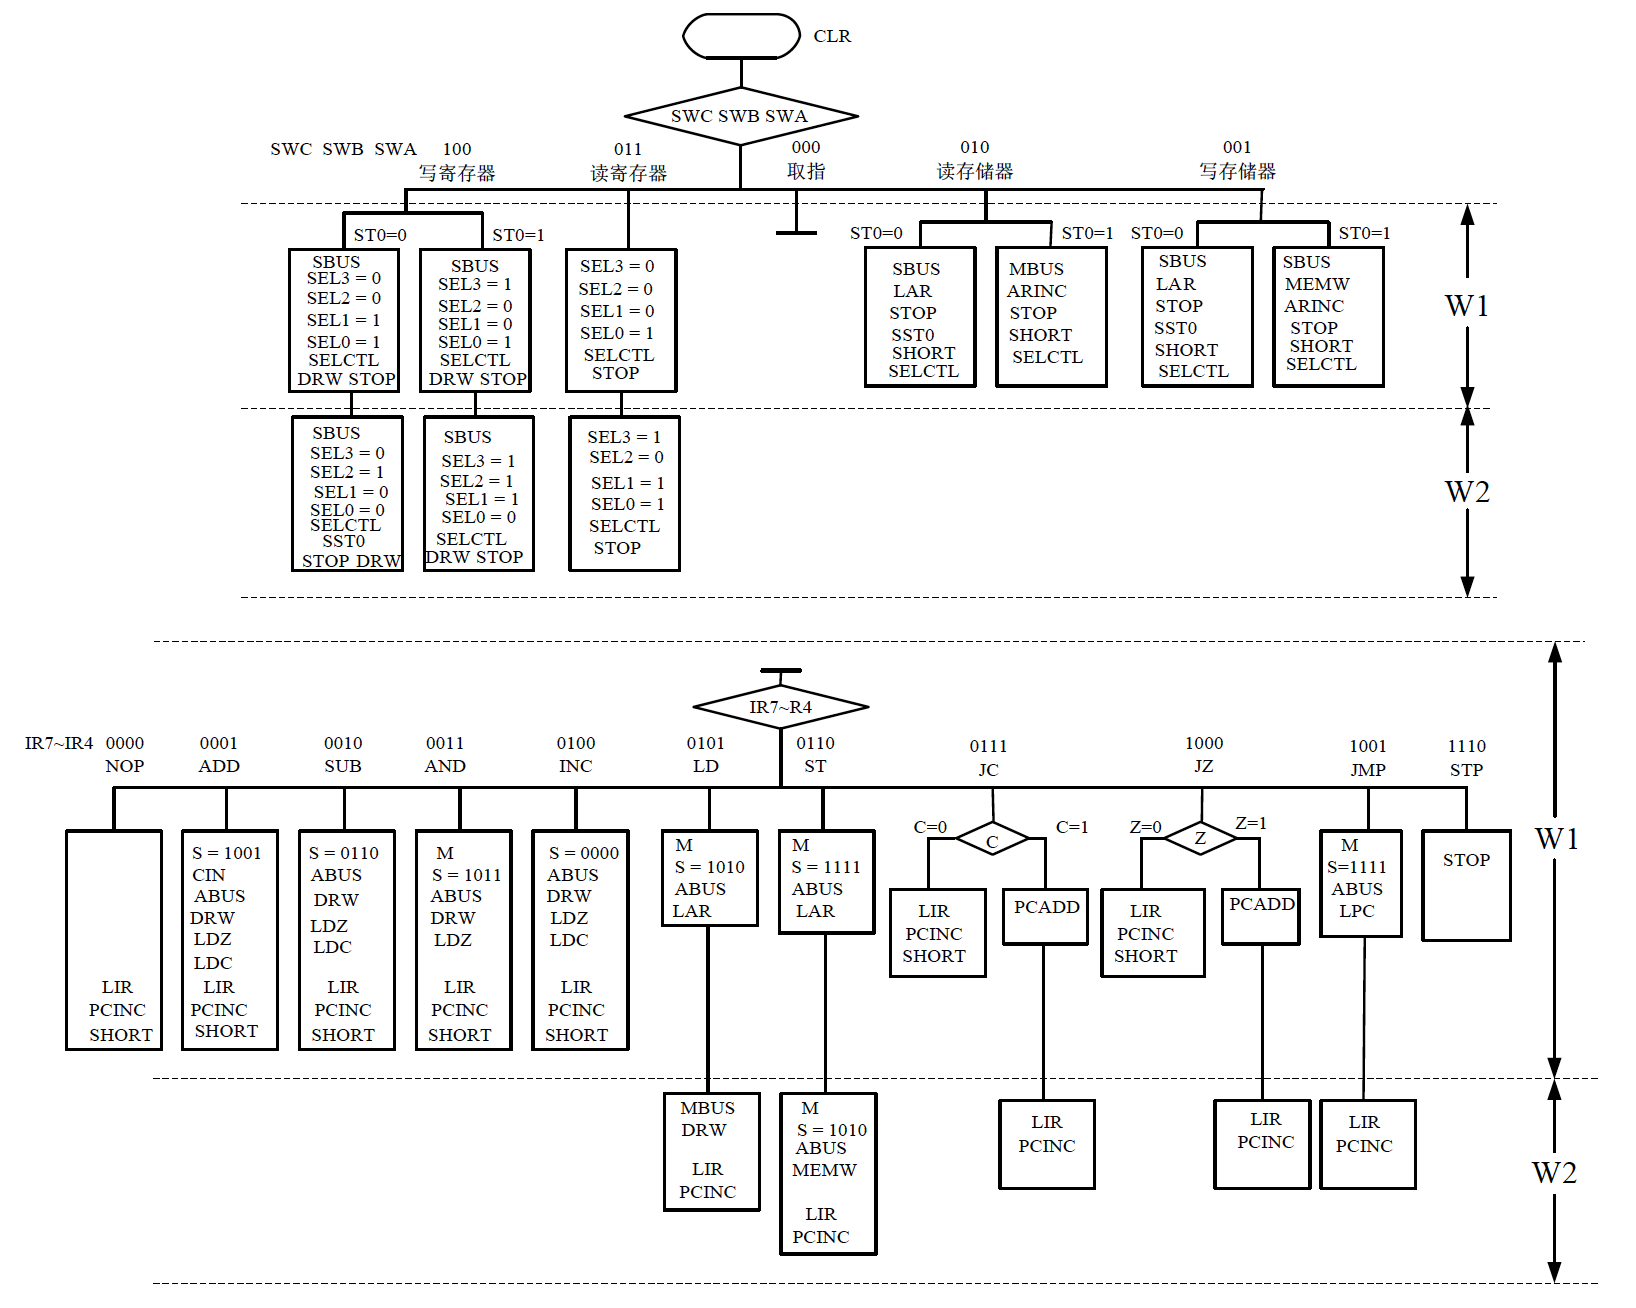
\includegraphics[width=1.0\textwidth]{流程图.png}
            	\caption{流水硬连线控制器参考流程图}
            	\centering
            	\label{fig:5-1-6}
            \end{figure}
            
    \subsection{添加指定 PC 指针的功能}
        现在我们来添加指定 PC 指针的功能,也就是我们可以指定程序从哪里开始执行。
        
        我们可以通过 $ST0$ 来实现这个功能,与我们在读写存储器里的操作类似。初始时 $ST0=0$,我们打开 $SBUS$ 和 $LPC$,将数据开关上的值存到 $PC$ 里,这就实现了指定程序首地址,同时我们将 $SST0$ 置为 $1$。在 $ST0=1$ 阶段我们就开始逐步执行我们的程序。流程图如 Figure\ref{fig:5-2} 所示。
        
        \begin{figure}[!ht]
            \centering
            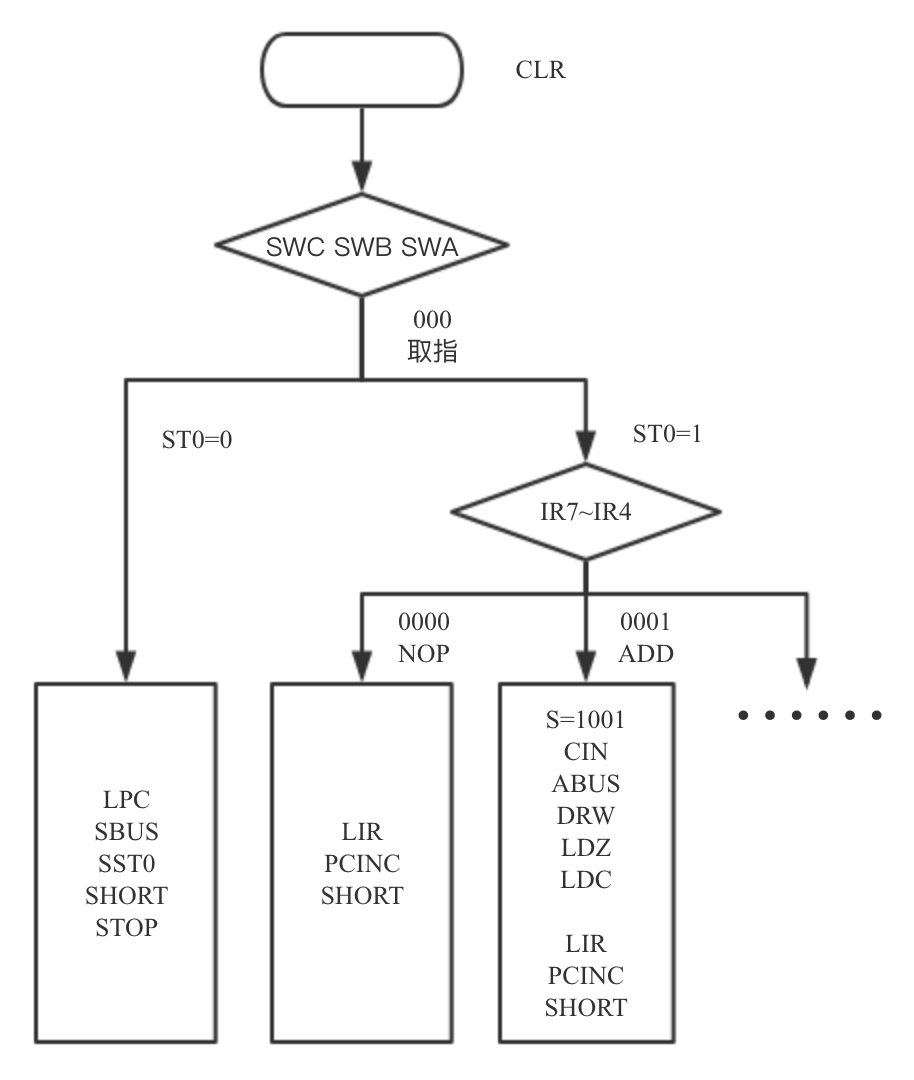
\includegraphics[width=0.6\textwidth]{PC指针.png}
            \caption{指定 PC 指针流程图}
            \label{fig:5-2}
        \end{figure}
        
    \subsection{扩充指令}
        在原指令的基础上,我们可以再扩展三条指令:XOR、OR、NOT,可以根据 ALU 的逻辑运算表来实现。由此我们可以画出流程图。如 Figure\ref{fig:5-3} 所示。
        
        \begin{figure}[!ht]
            \centering
            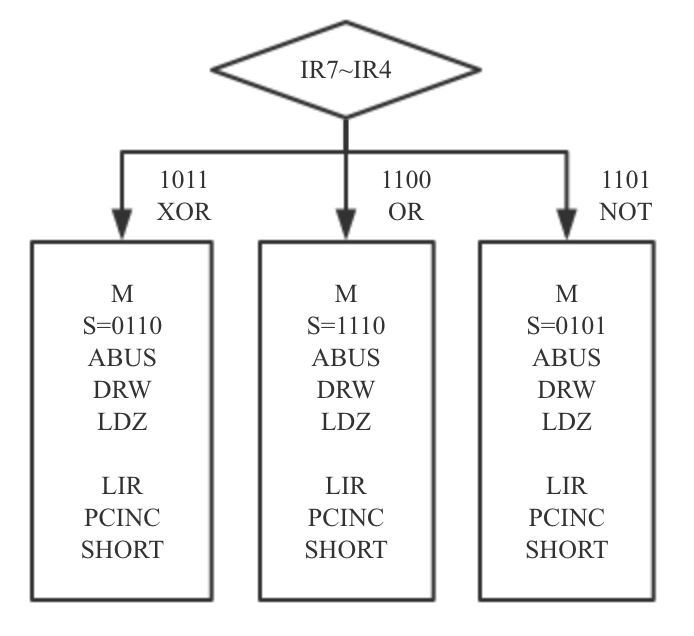
\includegraphics[width=0.6\textwidth]{扩指.png}
            \caption{扩充指令流程图}
            \label{fig:5-3}
        \end{figure}
        

    \subsection{组合逻辑译码表} 
        设计出硬连线流程图后,就可以设计译码电路。我们可以列出译码表,作为逻辑设计的根据。组合逻辑译码表如 Figure\ref{fig:5-4} 所示。需要注意的是,该表的前 $15$ 列,也就是所有的指令必须在 $ST0=1$ 的条件下执行,限于图片大小未在表中给出标注。
        
        \begin{figure}[!ht]
            \centering
            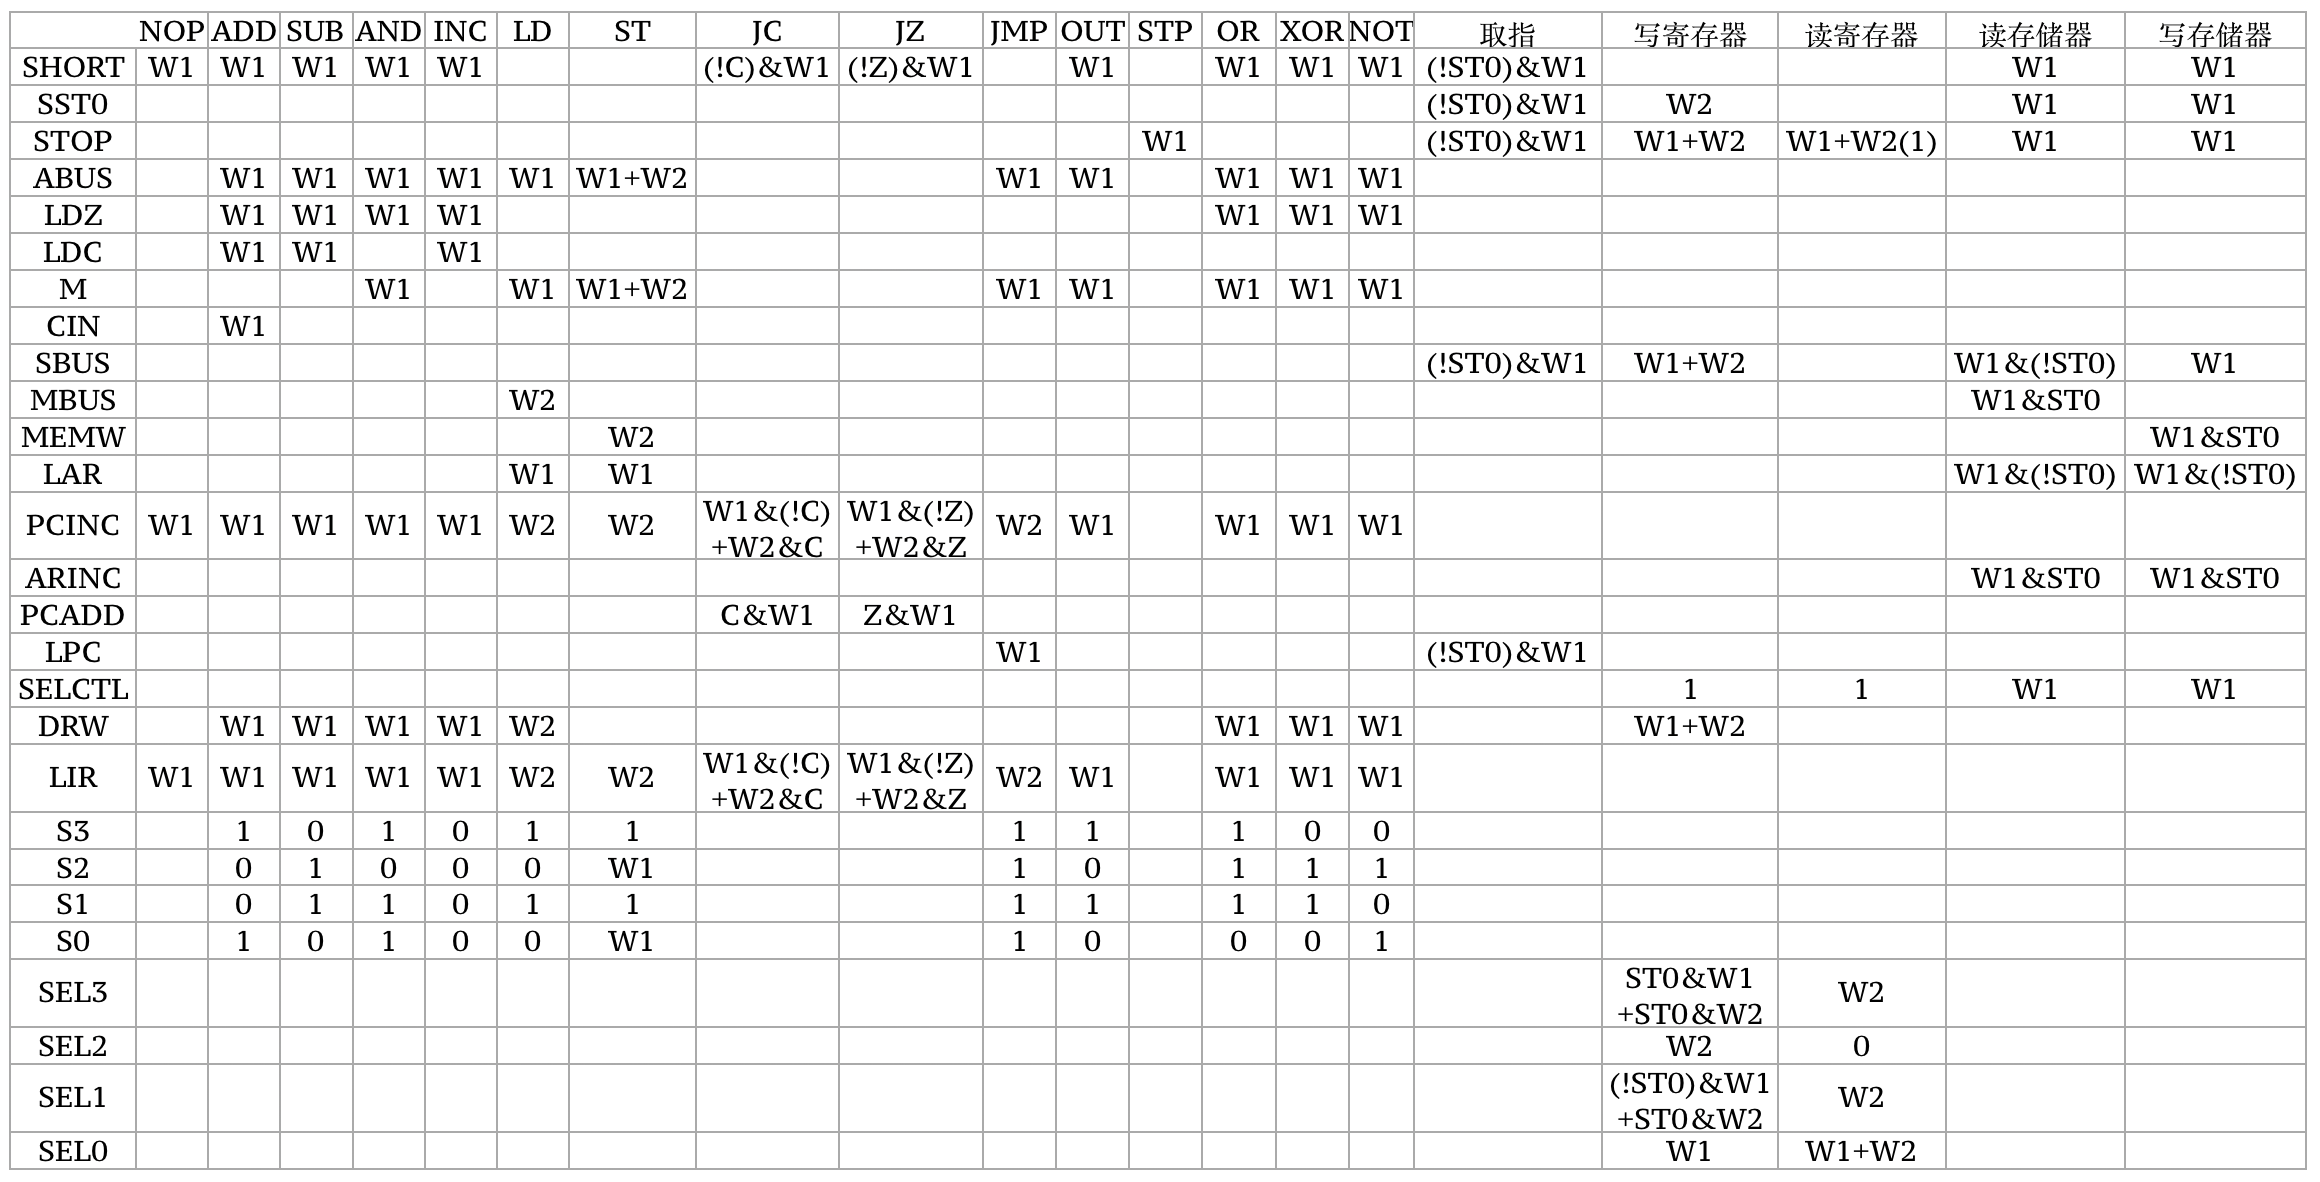
\includegraphics[width=1.0\textwidth]{组合逻辑译码表.png}
            \caption{组合逻辑译码表}
            \label{fig:5-4}
        \end{figure}
        
    \subsection{中断}
    最后我们可以来实现中断,中断是CPU 处理复杂指令必不可少的,比如其他程序运行时鼠标和键盘信息的输入,以及操作系统从用户态进入内核态调用方法……然而查阅芯片手册我们发现,在$EPM7128$中并没有中断相应操作的管脚供我们使用,所以我们无法在真机上运行。但是我们在这里提供了大致思路和实现流程,在以后有机会可以在提供相应管脚信号的芯片上验证实现。
    
        \subsubsection{原理}
        当有更高优先级的程序想要优先运行,CPU 需要找出一种方法,既能让高优先级程序尽快开始执行,又要在程序执行后继续之前(可能还没运行完的)程序。为了实现这个目的,CPU 将之前程序运行到哪儿保存下来,也就是保存$PC$当前指针,以及其他相关寄存器的值。之后$PC$读取中断向量,跳转到中断程序,当中断程序结束后,$PC$读取之前存储的指针,恢复相应寄存器的值,接着执行未执行完的程序。
        
        \subsubsection{需要新增的硬件}
        首先,要想保存现场,就需要一个寄存器来存储$PC$的值,并且在中断程序结束后恢复$PC$,这个寄存器就是$IAR$。我们也可以用存储器来代替寄存器,来存储$PC$的值以及其他与原来程序相关的寄存器值。
        
        \subsubsection{需要新增的信号}
        \begin{enumerate}
            \item \textbf{INT:}中断信号,若为1,则保存现场,进入中断程序;若为0,则继续运行。
            \item \textbf{INTDI:}禁止新的中断发生
            \item \textbf{INTEN:}允许中断的发生
            \item \textbf{LIAR:}保存当前地址(断点寄存器)
            \item \textbf{IABUS:}将$LIAR$中保存的地址打到总线上
        \end{enumerate}
        
        \subsubsection{需要新增的指令}
        \begin{enumerate}
            \item \textbf{DI:}关中断,$INTDI$
            \item \textbf{EI:}开中断,$INTEN$
            \item \textbf{IRET:}从中断程序返回,恢复现场,$IABUS$,$LPC$
        \end{enumerate}
        \subsubsection{中断运行过程}
        
        \begin{figure}
            \centering
            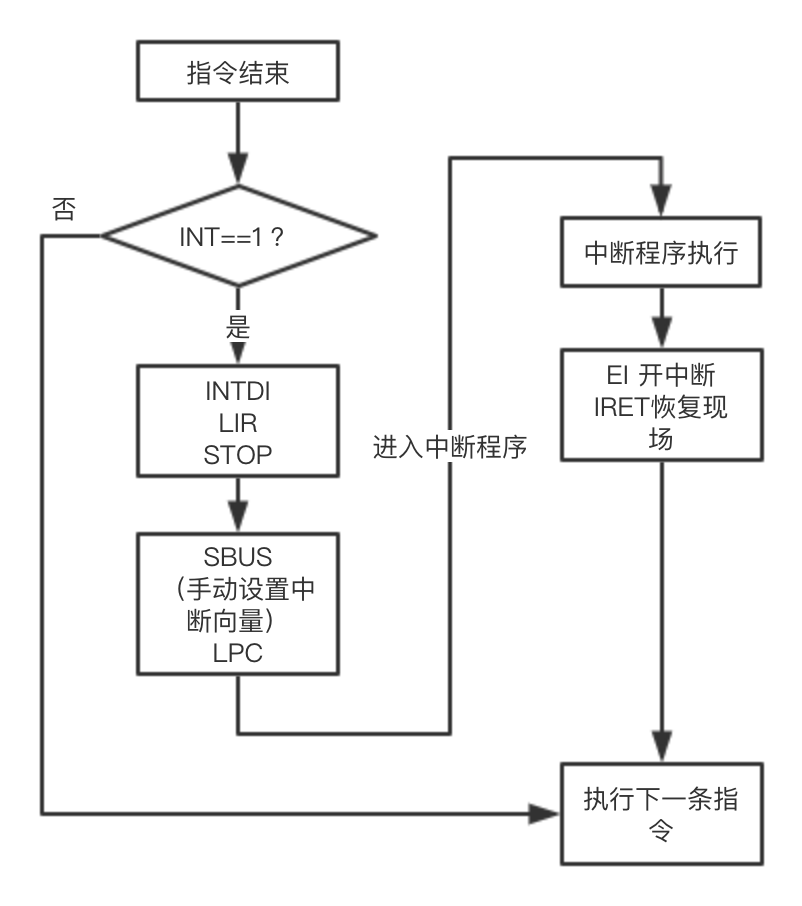
\includegraphics[width=0.6\textwidth]{中断流程图.png}
            \caption{中断流程图}
            \label{fig:int}
        \end{figure}
        
        如图\ref{fig:int}首先,设置$process$,让$INT$信号可以根据$INTDI$和$INTEN$来决定自己是否为1,之后在每条指令后判断$INT$是否为1,若为1,则执行$INTDI$和$LIAR$等保存现场和转到中断向量的指令,然后开始执行中断程序。
        
        在中断程序的末尾,需要有$IRET$指令,恢复现场,并恢复中断$EI$。
        
        \subsubsection{多级中断的想法}
        有关多级中断,首先,即使CPU开放了上述所说的相关引脚,我们也无法实现多级中断。因为我们只有
        一个$IAR$,也就只能保存一个现场。我们曾试想过用存储器来代替$IAR$存储多级中断的现场,在恢复现场的时候,将存储器中的指令地址打到数据总线中,再存入$PC$,但是这样还是需要保存在存储器中的地址,所以方法也不可行。大概还是需要更多硬件的支持才能实现多级中断吧。
        
\section{代码编写}
    有了流程图,编写代码的工作还是比较容易的,大体思路如下:
    
    首先对信号初始化。
    
    \begin{lstlisting}[language=vhdl]
        SHORT <= '0';
        LONG <= '0';
        CIN <= '0';
        SELCTL <= '0';
        ABUS <= '0';
        SBUS <= '0';
        MBUS <= '0';
        M <= '0';
        S <= "0000";
        SEL3 <= '0';
        SEL2 <= '0';
        SEL1 <= '0';
        SEL0 <= '0';
        DRW <= '0';
        SBUS <= '0';
        LIR <= '0';
        MEMW <= '0';
        LAR <= '0';
        ARINC <= '0';
        LPC <= '0';
        LDZ <= '0';
        LDC <= '0';
        STOP <= '0';
        PCINC <= '0';
        SST0 <= '0';
        PCADD <= '0';
    \end{lstlisting}
    
    然后判断如果按下了 CLR,就将 ST0 置为 0,否则进入我们的主程序。
    
    \begin{lstlisting}[language=vhdl]
        if (clr = '0') then
            ST0 <= '0';
        else
            ...
    \end{lstlisting}
    
    主程序的第一部分,如果 SST0 为 1,则在 T3 下降沿对 ST0 的值做出修改。
    
    \begin{lstlisting}[language=vhdl]
        if (T3'event and T3 = '0') and SST0 = '1' then
            ST0 <= '1';
        end if;
    \end{lstlisting}
    
    之后就通过 case 来判断 SWC~SWA,执行读存储器、写存储器、读寄存器、写寄存器、执行程序。
    
    \begin{lstlisting}[language=vhdl]
        case SWCBA is
            when "000" => 
                ...
            when "001" =>
                ...
            when "010" =>
                ...
            when "011" =>
                ...
            when "100" =>
                ...
        end case;
    \end{lstlisting}
    
    对于执行程序部分,我们依旧通过 case 来判断 IR7~IR4,执行不同的指令。
    
    \begin{lstlisting}[language=vhdl]
        case IRH is
            when "0000" => --NOP
                ...
            when "0001" => --ADD
                LIR <= W1;
                PCINC <= W1;
                SHORT <= W1;
                S <= "1001";
                CIN <= W1;
                ABUS <= W1;
                DRW <= W1;
                LDC <= W1;
                LDZ <= W1;

            when "0010" => --SUB
                ...
        end case;
    \end{lstlisting}
    
    代码的大致结构就是这样,详细代码见附录。
    
\section{调试过程}
    不同于以往的软件调试,这里我们不仅需要在 EDA 软件上成功编译,
    更重要的是将设计下载到 EPM7128 器件中,在真实的环境下运行并调试。
    
    首先需要检查 TEC-8 控制台是否工作良好,接下来下载我们编译好的
    程序,以单拍方式(DP=1)执行编排好的验证程序,通过检查
    数据、指令和信号的指示灯来验证程序的正确性。
    
    \subsection{验证程序 1}
        验证程序 1 如 Figure\ref{fig:6-1} 所示。
        
        \begin{figure}[!ht]
            \centering
            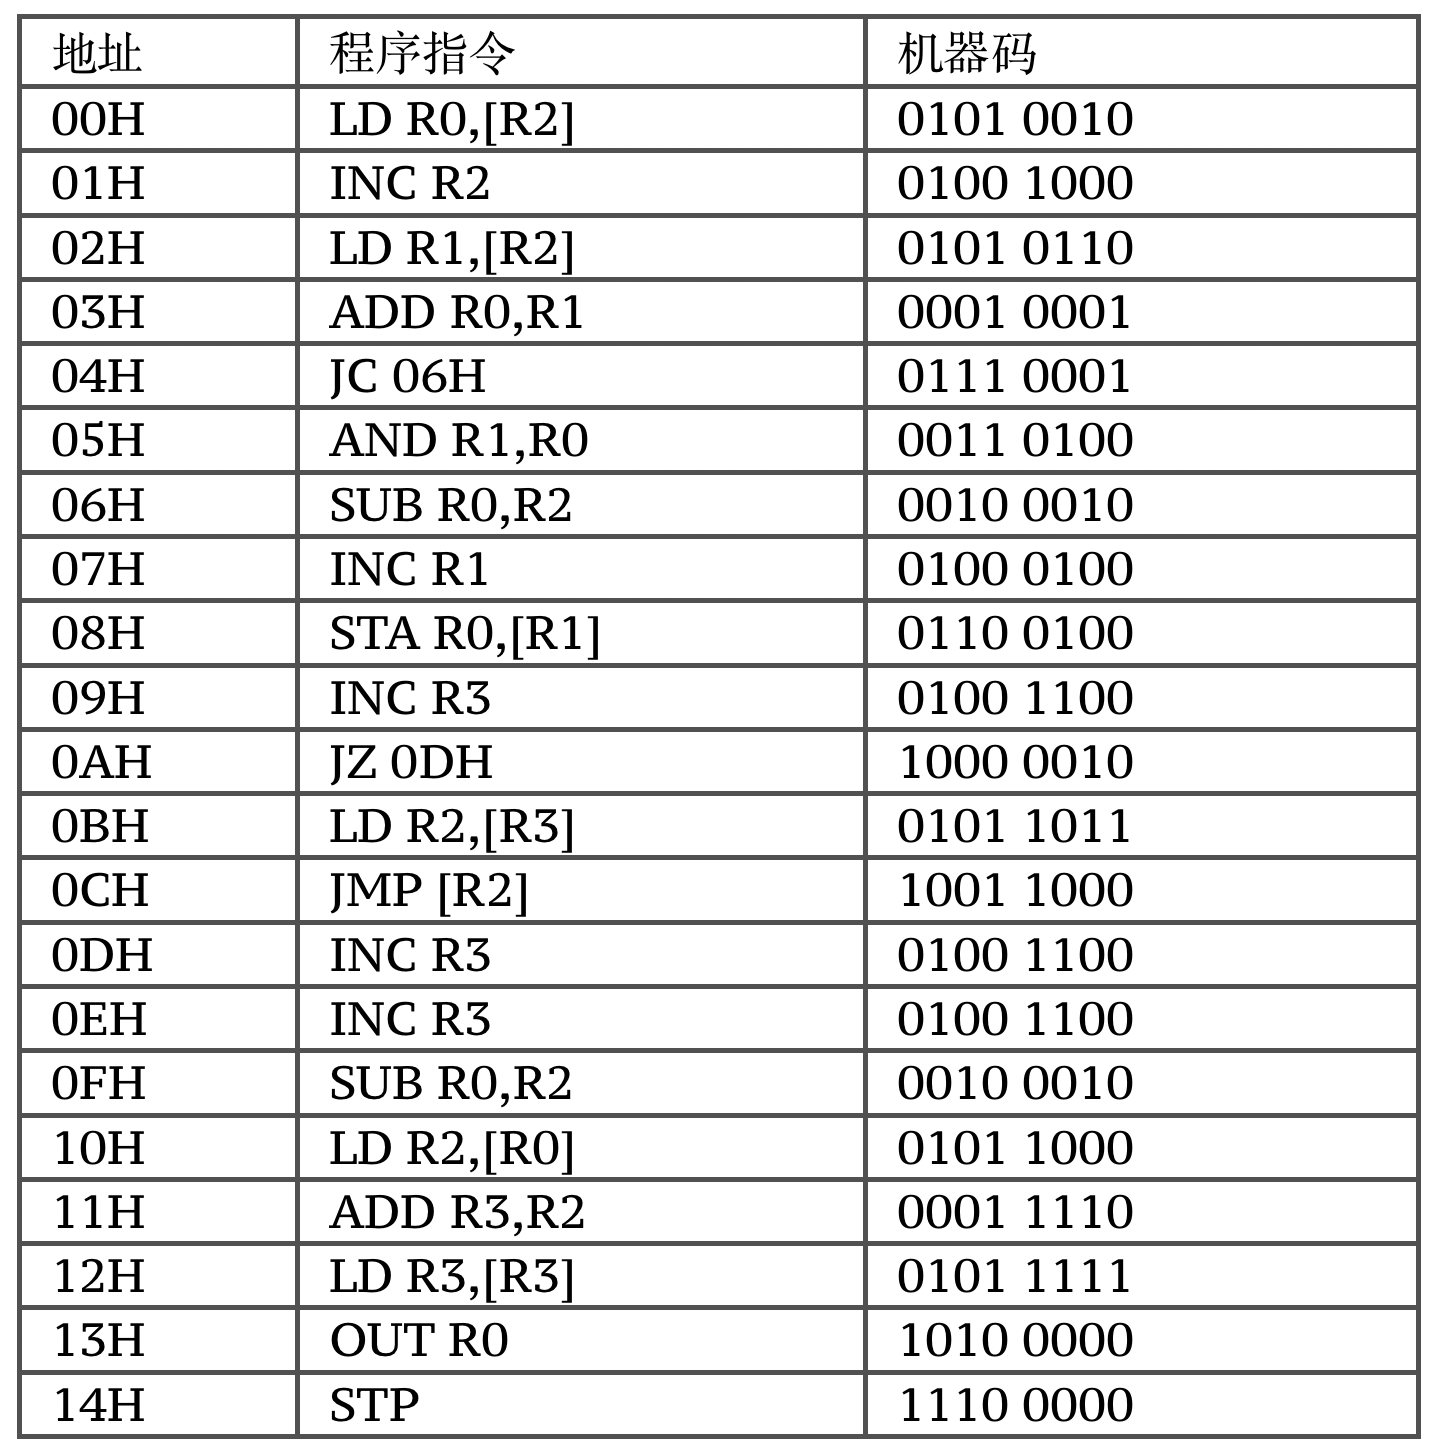
\includegraphics[width=0.9\textwidth]{测试程序.png}
            \caption{验证程序 1}
            \label{fig:6-1}
        \end{figure}
        
        程序运行前,规定寄存器 $R2=60H$,$R3=FDH$;存储器 $[60H]=67H$,$[61H]=80H$,$[62H]=FDH$,$[80H]=60H$,$[FEH]=03H$,$[FFH]=03H$。
    
        我们来手动模拟一下程序的运行过程:
        
        \begin{enumerate}
            \item \verb"LD R0,[R2]",$R0\gets [60H]=67H$
            \item \verb"INC R2",$R2\gets 61H$
            \item \verb"LD R1,[R2]",$R1\gets [61H]=80H$
            \item \verb"ADD R0,R1",$R0\gets R0+R1=E7H$
            \item \verb"JC 06H",无进位,不跳转
            \item \verb"AND R1,R0",$R1\gets R1\&R0=80H$
            \item \verb"SUB R0,R2",$R0\gets R0-R2=86H$
            \item \verb"INC R1",$R1\gets 81H$
            \item \verb"ST R0,[R1]",\dotuline{$[81H]\gets 86H$}
            \item \verb"INC R3",$R3\gets FEH$
            \item \verb"JZ 0DH",不为 $0$,不跳转
            \item \verb"LD R2,[R3]",$R2\gets [FEH]=03H$
            \item \verb"JMP [R2]",跳转到 $[03H]$
            \item \verb"ADD R0,R1",$R0\gets R0+R1=07H$
            \item \verb"JC 06H",有进位,跳转到 $[06H]$
            \item \verb"SUB R0,R2",$R0\gets R0-R2=04H$
            \item \verb"INC R1",$R1\gets 82H$
            \item \verb"ST R0,[R1]",\dotuline{$[82H]\gets 04H$}
            \item \verb"INC R3",$R3\gets FFH$
            \item \verb"JZ 0DH",不为 $0$,不跳转
            \item \verb"LD R2,[R3]",$R2\gets [FFH]=03H$
            \item \verb"JMP [R2]",跳转到 $[03H]$
            \item \verb"ADD R0,R1",$R0\gets R0+R1=86H$
            \item \verb"JC 06H",无进位,不跳转
            \item \verb"AND R1,R0",$R1\gets R1\&R0=82H$
            \item \verb"SUB R0,R2",$R0\gets R0-R2=83H$
            \item \verb"INC R1",\dotuline{$R1\gets 83H$}
            \item \verb"ST R0,[R1]",\dotuline{$[83H]\gets 83H$}
            \item \verb"INC R3",$R3\gets 00H$
            \item \verb"JZ 0DH",为 $0$,跳转到 $[0DH]$
            \item \verb"INC R3",$R3\gets 01H$
            \item \verb"INC R3",$R3\gets 02H$
            \item \verb"SUB R0,R2",\dotuline{$R0=R0-R2=80H$}
            \item \verb"LD R2,[R0]",\dotuline{$R2\gets [80H]=60H$}
            \item \verb"ADD R3,R2",$R3\gets R3+R2=62H$
            \item \verb"LD R3,[R3]",\dotuline{$R3\gets [62H]=0FDH$}
            \item \verb"OUT R0",输出 $80H$
            \item \verb"STP",程序结束
        \end{enumerate}
        
        最后,我们的寄存器 $R0=80H$,$R1=83H$,$R2=60H$,$R3=FDH$;存储器 $[81H]=86H$,$[82H]=04H$,$[83H]=83H$(上述寄存器和存储单元的最后一次操作已在上述过程中标出)。可以通过读寄存器和读存储器操作来检查结果是否符合预期。

    \subsection{验证程序 2}
        验证程序 2 如 Figure\ref{fig:6-2} 所示。通过该程序我们可以验证扩指和 PC 的功能。
        
        \begin{figure}[!ht]
            \centering
            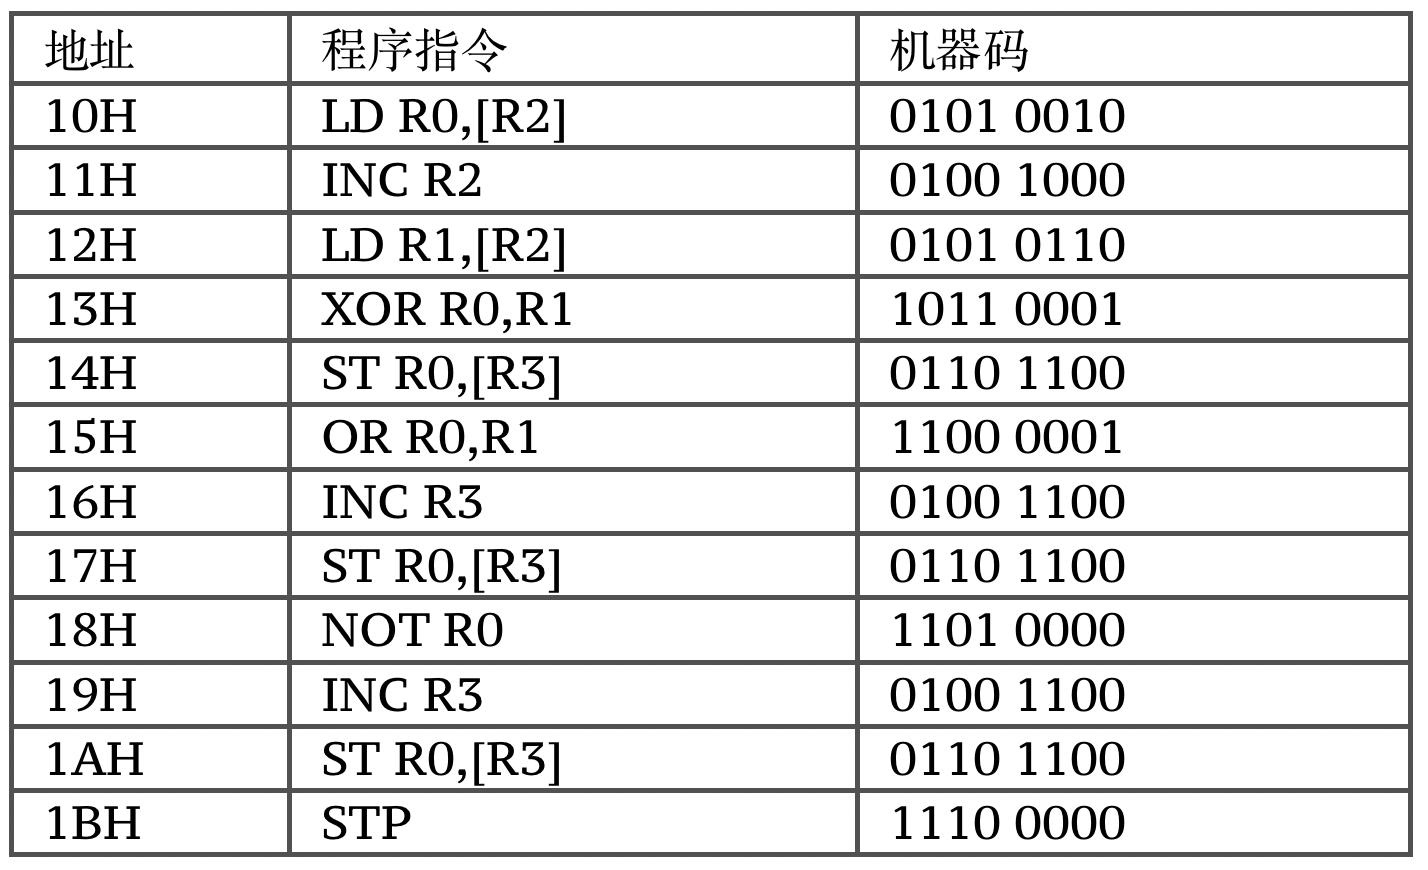
\includegraphics[width=0.9\textwidth]{测试程序2.png}
            \caption{验证程序 2}
            \label{fig:6-2}
        \end{figure}
        
        程序运行前,规定寄存器 $R2=60H$,$R3=80H$;存储器 $[60H]=67H$,$[61H]=80H$。注意到我们需要将程序运行的起始位置设置为 $10H$。
        
        我们来手动模拟一下程序的运行过程:
        
        \begin{enumerate}
            \item \verb"LD R0,[R2]",$R0\gets [60H]=67H$
            \item \verb"INC R2",$R2\gets 61H$
            \item \verb"LD R1,[R2]",$R1\gets [61H]=80H$
            \item \verb"XOR R0,R1",$R0\gets R0\ xor\ R1=E7H$
            \item \verb"ST R0,[R3]",$[80H]\gets R0=E7H$
            \item \verb"OR R0,R1",$R0\gets R0+R1=E7H$
            \item \verb"INC R3",$R3\gets 81H$
            \item \verb"ST R0,[R3]",$[81H]\gets R0=E7H$
            \item \verb"NOT R0",$R0\gets !R0=18H$
            \item \verb"INC R3",$R3\gets 82H$
            \item \verb"ST R0,[R3]",$[82H]\gets R0=18H$
            \item \verb"STP",程序结束
        \end{enumerate}
        
        最后,我们的存储器 $[80H]=E7H$,$[81H]=E7H$,$[82H]=18H$。
        
    \subsection{调试过程中的问题}
        在验证过程中,我们遇到了如下问题,经过探讨与实践,我们的问题得到了解决。
        
        \subsubsection{问题 1:节拍信号和节拍脉冲}
            见 4.1.1 所示。
        \subsubsection{问题 2:为什么一个指令要通过 $W1$ 和 $W2$ 两个节拍信号来实现?}
            比如$ST$指令这样的需要读写存储器的指令,读写存储器是一项很费时间的工作,可能需要占用两三个节拍脉冲的时间,这时候一个节拍电位已经无法提供后面的打入寄存器等操作的节拍脉冲了,所以把它放到下一个节拍信号当中。
            
            还有一种可能就是跳转命令,在跳转命令当中,我们需要把$PC$更新之后再跳转到$PC$指向的指令,这时也无法用一个节拍电位提供的三个节拍脉冲实现。
            
        \subsubsection{问题 3:在减法运算中,进位标志 $C$ 是如何变化的?}
            74181 对减法运算采用的是补码运算方式,即先求得[-减数]的补码,然后和被减数的补码相加的方式完成。因此一个较大的数减去一个较小的数,或者 2 个相等的数相减时产生进位。
        \subsubsection{问题 4:中断当中,如何读取 $PC$?}
            查阅发现需要用$LIAR$信号将$PC$的值读取到$LIR$当中,本次实验所用芯片没有这个信号的管脚。
        \subsubsection{问题 5:$T3$ 是干啥的}
            $T3$是三个节拍脉冲中的一个,用于打入寄存器和其他需要时序的操作。
        \subsubsection{问题 6:没写在 $T3$ 下降沿就改变 $ST0$,程序无法正常运行}
            如果这里不用时序信号而用节拍信号的话,不能保证 $ST0$ 的值在该节拍结束后才改变,从而导致某些其他信号的值可能发生变化。
        \subsubsection{问题 7:如何让每条指令执行结束后才检测中断?}
            在微程序控制器实验中,每条指令运行之后可以检测有无中断的产生。但在硬连线控制器当中,我们可以设置$process$,让$INT$信号可以根据$INTDI$和$INTEN$来决定自己是否为1,之后在每条指令后判断$INT$是否为1,若为1,则执行$INTDI$和$LIAR$等保存现场和转到中断向量的指令,然后开始执行中断程序。
        \subsubsection{问题 8:如果在指令执行中中断,是不是还要记录节拍电位?如何恢复?}
            目前还没有找到在指令中中断的方法,暂且使用在每次指令结束后判断是否需要中断,保存现场和转到中断程序的方法。
        \subsubsection{问题 9:将编译好的程序下载到 TEC-8 的时候提示 Error: Operation failed}
            换了一根下载线后成功了。
        \subsubsection{问题 10:初始时 $INS7\sim INS0$ 显示奇怪的信号}
            由于 $INS7\sim INS0$ 显示的是 $PC$ 指向内存单元的指令,初始时 $PC$ 指向的单元可能存储着先人留下的指令。
        \subsubsection{问题 11:单拍可以正确执行,但连续无法正确执行}
            换了一个实验台成功了。
        \subsubsection{问题 12:验证程序第12条指令后没有跳转到13条指令,而是直接到NOP}
            可能原因是出现了毛刺导致指令跳转失败。换一台试验台,重新录入指令,就很顺利地获得了结果。
            
            
    
    \subsection{调试小结与心得}
    和软件编写很不一样,在这里编译成功只是万里长征的第一步,
    只有将自己的代码放到真实的硬件上,并用心地为它编排测试程序,
    在应用中慢慢锤炼,才能让自己的代码更加完美。

\section{工作日志}
    \subsection{4 月 1 日(房庆凯记)}
        今天是第一次来机房做实验,时隔好几个月又一次接触实验台,感觉还有些生疏。翻出了上学期数据通路实验的 PPT、大一时 VHDL 语言的 PPT、TEC-8 指导手册,第一次来我们不着急开始做实验,第一件事是先把所有的基础知识都回忆起来,基础牢固了以后做实验也会顺利一些。
        
        首先打开了熟悉的数据通路那张大图,我们手动模拟了一遍程序运行的整个流程。在这个过程中,我们发现甚至有很多信号的含义都已经记不清了,对照着手册,我们终于搞清楚了这张图,脑海里有了一个大致的图景。
        
        接下来,我们决定就一步一步来,就从最简单的非流水做起吧。通过查阅手册,我们找到了一张硬连线非流水的流程图开始研究,研究过程中我们发现除了刚才数据通路图上的之外,还有一些辅助信号,比如 ST0、SST0 等,经过讨论我们也搞清楚了这些信号的意义,然后又挨个框研究,每个框里为什么是这几个信号等等,最终我们搞清楚了流程图,大体思路已经逐步浮现出水面了。
        
        对照流程图我们开始搞组合逻辑译码表,经过两个人的合作和反复检查,最后终于将这张大表搞出来了!
    
    \subsection{4 月 8 日(陈政瑞记)}
        上次来我们基本搞清楚了所有的理论,于是今天我们准备开始上机编码了。简单复习了一下 VHDL 的语法,我们便开始了上机编程。
        
        有了流程图的参考,编写代码相对来说还是比较顺利。使用 VHDL 的 case 语句可以很好的描述出程序的结构。大概花了半个多小时的时间,第一版代码完成了!
        
        然后我们开始对照着管脚表分配管脚,一个人念一个人写,很快完成了这项工作。
        
        接下来的工作就是把代码烧到实验台上,这里我们还是遇到了一些小问题,中间好几次提示 Error,Google了一下Error的描述,在不知道哪所大学的PPT里面发现,可能是硬件的型号不对。我们检查了一下代码绑定的硬件型号之后,又发现我们用的试验台和其他桌子上的试验台颜色有些不一样,于是我们选择换了一个试验台继续试验。在排除了试验台的差异之后,依旧烧录不上,我们又发现线的两个指示灯都是红色的,原来是线的问题导致,换了几次线后便成功了。
        
        拿出了上学期 PPT 上的那个简单的验证程序,我们跑了一下,结果很遗憾并没有一次成功。不过我们这次没有怀疑箱子,就反复检查了几遍代码,后来发现是代码中有一个地方的时序信号写成了电平信号,改完之后成功了!
        
    \subsection{4 月 15 日(房庆凯记)}
        上周的成功给我们带来了极大的信心,今天我们决定开始尝试流水了。
        
        之前一直没有研究这里的流水是什么意思,以为十分高深。今天我们两个人研究了一下,发现不过就是在执行程序的时候,每次执行一条指令就顺带把下一条指令取出来。也就是说对应到代码上我们只需要修改一下执行程序部分的组合逻辑。有了非流水的经验,改成流水还是相对比较容易的,与此同时我们又修改了组合逻辑译码表和我们的代码,按照之前的流程开始测试代码。竟然取得了一次成功!
    \subsection{4 月 22 日(陈政瑞记)}
        到上周为止,这次实验的基本要求我们已经完成的差不多了。现在开始实现附加功能:扩指和 PC。
        
        所谓扩指其实很简单,对照着 ALU 的逻辑运算表就可以了,我们添加了 XOR、OR、NOT 三条指令,这一部分我们很快完成了。与此同时,我们扩充了我们的组合逻辑译码表(见图\ref{fig:5-4})。
        
        PC 也就是指定程序运行的首地址,这个其实也比较好实现,就是在我们程序运行之前,执行一次 LPC。当时代码上我们思考了两种实现方式:第一种是再加一个 $SWC\sim SWA$ 的取值,专门用来指定 PC;第二种是依旧在 $SWC\sim SWA=000$ 里面,然后用 ST0 来区分指定 PC 和执行程序的过程。最后我们选择了第二种方式。
        
        这里的代码编写还是比较容易实现的,在判断 $SWC\sim SWA=000$ 后,根据 ST0 的值判断执行哪部分代码就可以了。
        
        最后我们自己手动编写了一个验证程序,可以验证我们新添加的指令以及 PC 功能,不出所料,最后的结果和我们之前预想的完全一致,成功了~
        
    \subsection{5 月 6 日(房庆凯记)}
        上段时间老师发了一个验证程序,今天我们决定来测试一下。
        
        首先我们手动模拟了一下这个验证程序,程序虽短,抵不住来回跳转。不得不说老师这个程序设计的十分精妙。通过这个程序我们几乎验证了所有指令的正确性,最后通过检查寄存器和存储器的值,发现和老师给出的结果以及我们手算的结果均一致,看来我们的程序还是没有什么问题的。
        
        不过在验证过程中,我们的试验台出现了问题,导致我们验证程序执行第12条指令后无法进入第13条指令。听说其他同学也遇到了这个情况,可能原因是出现了毛刺导致指令跳转失败。我们换了一台试验台,重新录入指令,再运行就很顺利地获得了结果。
        
    \subsection{5 月 13 日(陈政瑞记)}
        最后我们想尝试一下中断。
        
        回忆上学期的中断实验,我们是用微程序控制器(现在想想微程序的实验真是简单,不需要自己写代码,摁开关就行),所以我们先翻出PPT,回忆了一下微程序上中断的流程。
        
        然后我们对照着硬连线流水的现实环境,看一看能不能实现硬连线环境下的流水。发现,首先是好多信号没有管脚的分配,就像$INT$,$LIAR$等。我们想能否用打到存储器的方法来代替保存现场,后来发现根本没有取出$PC$当前值的方法。所以我们认为以当前的实验环境没法实现中断。后来询问其他同学之后,我们也肯定了这一想法。
        
    \subsection{5 月 20 日(房庆凯记)}
        这周就要验收了,于是我们决定再来熟悉一遍整个流程。
        
        于是我们重新建了一个 project,然后添加进之前我们的代码,重新分配管脚、重新烧制程序。这个过程中我们遇到了许多熟悉的问题,但是有了之前的经验,我们还是轻松的解决了。
        
        这次实验基本就这么完成了,之后的工作便是整理实验报告了。
    
\section{心得体会}
    \subsection{房庆凯}
    	随着验收的到来,这次的课程设计也接近了尾声,看着自己做出的结果在 TEC-8 实验台上成功运行,心中生发了许多感想。
    	
	第一次接触 TEC-8 还是在一年前的数字逻辑课上,当时打开实验台的感觉就是:满满当当的开关、指示灯,这也太麻烦了吧!后来在老师的指导下,一步步开始了我们的实验。从最基本的门电路开始,紧接着是组合逻辑、时序逻辑……电路越来越复杂,需要连的线越来越多,随之而来的是错误的出现。为了寻找一个错误,可能需要用逻辑测试笔挨个接口排查很久。
	
	下半年的组成原理课,再次见到了熟悉的 TEC-8,然而这次的实验比起之前的数字逻辑可以说更加复杂,越来越多的信号、越来越多的连线,每次实验仅仅连线就要准备好久。也是在这个时候第一次见到了数据通路的那张大图,老师用教杆指着,数据从哪儿走到哪儿、哪个信号打开、哪个信号关上……相信有许多同学和我一样,被这张图“折磨”了好久也没有真正搞清楚这张图的含义。但是好心的老师把怎么连线、怎么操作都告诉了我们,最后虽然有些原理还是模棱两可,但还是完成了运算器、存储器、数据通路、微程序、中断等实验。
	
	于是这个学期再次与 TEC-8 见面了,这次与以往不同。老师布置完任务,之后的一切都要靠自己了。刚拿到任务的时候依然是一头雾水,不知道从何做起。眼前的这个实验台令人感到熟悉而又陌生。这次的任务是做一个流水硬连线控制器,拿到任务时:硬连线是什么?流水又是如何实现的?虽然我知道这个实验与上学期的微程序有异曲同工之处,但上学期留下的模糊印象并没有给我什么帮助,于是我决定从头开始认真研究。
	
	再次拿出数据通路那张大图以及硬连线的流程图,第一件事是一个不落的搞清楚每个信号的含义,然而这项工作也没有我想象中的那么容易。比如经常有“在Ti上升/下降沿”的字眼,这是什么意思?节拍信号和节拍脉冲又有什么关系?搞清楚这些问题后,我又手动模拟了写存储器、读存储器、写寄存器、读寄存器、取指各个过程,数据是怎么在总线上流动的?哪些信号需要有效?哪些信号应该无效?经过反复查阅资料、与同学讨论,这些问题都一步步得到了解决,课程设计的题目也不再那么深不可测。
	
	接下来开始流水,发现流水也没有想象中的那么麻烦,只是在执行指令的同时取出下一条指令,修改一下硬连线的组合逻辑就可以实现。之后,根据流程图写出每个信号在每条指令中的有效条件,写出 VHDL 的每一句代码……每一项工作都需要十足的细心、耐心才能正确完成。每次完成一项工作,我都会与我的搭档反复检查,确认无误后再进行下一项工作。之后添加 PC 和扩指的功能,经过我们的讨论,问题也迎刃而解。
	
	一直以来我都秉持着“Think twice, code once”的思想,准备工作做足了之后,代码编写真的没有那么难。然而,写完 VHDL 代码只是成功的第一步。把代码烧到实验台上之后,我们的实验才刚刚开始。实验过程中,我们遇到过软件的问题,也遇到过硬件的问题。每次遇到问题,和我的搭档一起分析错误现象,寻找解决方法。最后我们几经修改代码、换实验台,终于让程序顺利的跑了起来。编制进老师提供的以及我们自己编写的验证程序,每次按一下 QD,各个指示灯的变化均在我们的预料之中,最后从存储器和寄存器中读出的数字也与期望一致,看到最后的结果,我们深感欣慰。
	
	回过头来再看看 TEC-8,发现它不再那么令人感到恐惧,反倒感觉它已经在我的掌控之中。我也不像刚拿到题目时一头雾水,对验收充满恐惧,因为现在的我对实验台上每个指示灯的含义、流程图中每个信号的含义、每条指令对应的有效信号、代码中的每一条语句都已经深刻理解。如果要在最后谈一下做完这次课程设计的感受,最直接的感受就是复杂,复杂不是因为逻辑上有难以理解的地方,而是因为信号多、指令多、组合逻辑各有不同,如果没有足够的细心和耐心一定无法完成!克服掉这一切困难后的感受,就是真的非常有收获!对组成原理这一套理论的理解达到了一个全新的、更加系统的高度,在实验中也积累了发现问题、解决问题的方法,这些都是我在上学期做微程序时没有得到的收获。总之,这次课程设计在我的计算机硬件学习之路上有着非凡的意义!
	
    \subsection{陈政瑞}
    \begin{enumerate}
        \item \textbf{起步:}着手开始实验时,最好的方法不是先把所有相关知识都搞地分毫不差,而是奔向实验室,先扳起来开关再说。边做边学,不仅可以有效防止拖延症,而且带着问题学习可以把知识掌握得更扎实。
        \item \textbf{实验中:}开始做实验了,就要把每个不懂的地方搞明白,最好把不懂的地方按照层次和流程记一下,一些地方先默认是对的,一部分整体整体搞清楚了再回过头来看这些细节。有时候一点细节的地方可能就是一个潜藏的bug
        \item \textbf{沟通交流:}和其他同学多多交流,可以起到$1+1>2$的效果。有很多操作上的坑,知道了就可以避免,不知道就会很苦恼,这时候和其他同学讨论一下,可能就会发现自己操作上的低级错误。自己遇到的坑也能分享出去,让更多人避免踩坑。
        \item \textbf{搭档:}单独研究自己琢磨的时候就很累,但跟搭档一起讨论问题的时候就很欢乐,就像运行一条指令,我取出来指令,搭档就接着打到寄存器里,互相将思路连接起来,累了还会扯皮…总之就是比较高兴地做实验。不过也要注意控制好分工做和一起做的比例,因为一起做大部分都是两个人在做同一件事,总体效率可能会降低。
        \item 实验室去多了感觉自己大脑回路在向CPU回路发展,见图\ref{fig:4-1-2}
    \end{enumerate}
    
\section{附录}
    \subsection{源代码}
        \begin{lstlisting}[language=vhdl]
library ieee;
use ieee.std_logic_1164.all;
use ieee.std_logic_unsigned.all;

entity yycpu is
    port (
        SWC, SWB, SWA, clr, C, Z, W1, W2, W3, T3, QD : in std_logic;
        IRH : in std_logic_vector(3 downto 0);
        SELCTL, ABUS, M, SEL3, SEL2, SEL1, SEL0, DRW, SBUS, LIR, MBUS, MEMW, LAR, ARINC, LPC, PCINC, PCADD, CIN, LONG, SHORT, STOP, LDC, LDZ : out std_logic;
        S : out std_logic_vector(3 downto 0)
    );
end yycpu;

architecture arc of yycpu is
    signal SWCBA : std_logic_vector(2 downto 0);
    signal ST0, SST0 : std_logic;
begin
    SWCBA <= SWC & SWB & SWA;

    process (SWCBA, IRH, W1, W2, W3, ST0, C, Z, clr, T3)
    begin
        SHORT <= '0';
        LONG <= '0';
        CIN <= '0';
        SELCTL <= '0';
        ABUS <= '0';
        SBUS <= '0';
        MBUS <= '0';
        M <= '0';
        S <= "0000";
        SEL3 <= '0';
        SEL2 <= '0';
        SEL1 <= '0';
        SEL0 <= '0';
        DRW <= '0';
        SBUS <= '0';
        LIR <= '0';
        MEMW <= '0';
        LAR <= '0';
        ARINC <= '0';
        LPC <= '0';
        LDZ <= '0';
        LDC <= '0';
        STOP <= '0';
        PCINC <= '0';
        SST0 <= '0';
        PCADD <= '0';

        if (clr = '0') then
            ST0 <= '0';
        else
            if (T3'event and T3 = '0') and SST0 = '1' then
                ST0 <= '1';
            end if;

            case SWCBA is
                when "000" => 
                    if ST0 = '0' then
                        LPC <= W1;
                        SBUS <= W1;
                        SST0 <= W1;
                        SHORT <= W1;
                        STOP <= W1;
                    else
                        case IRH is
                            when "0000" => --NOP
                                LIR <= W1;
                                PCINC <= W1;
                                SHORT <= W1;

                            when "0001" => --ADD
                                LIR <= W1;
                                PCINC <= W1;
                                SHORT <= W1;
                                S <= "1001";
                                CIN <= W1;
                                ABUS <= W1;
                                DRW <= W1;
                                LDC <= W1;
                                LDZ <= W1;

                            when "0010" => --SUB
                                LIR <= W1;
                                PCINC <= W1;
                                SHORT <= W1;
                                S <= "0110";
                                ABUS <= W1;
                                DRW <= W1;
                                LDC <= W1;
                                LDZ <= W1;

                            when "0011" => --AND
                                LIR <= W1;
                                PCINC <= W1;
                                SHORT <= W1;
                                S <= "1011";
                                M <= W1;
                                ABUS <= W1;
                                DRW <= W1;
                                LDZ <= W1;

                            when "0100" => --INC
                                LIR <= W1;
                                PCINC <= W1;
                                SHORT <= W1;
                                S <= "0000";
                                ABUS <= W1;
                                DRW <= W1;
                                LDC <= W1;
                                LDZ <= W1;

                            when "0101" => --LD
                                LIR <= W2;
                                PCINC <= W2;
                                S <= "1010";
                                M <= W1;
                                ABUS <= W1;
                                LAR <= W1;
                                MBUS <= W2;
                                DRW <= W2;

                            when "0110" => --ST
                                LIR <= W2;
                                PCINC <= W2;
                                M <= W1 or W2;
                                S(3) <= '1';
                                S(2) <= W1;
                                S(1) <= '1';
                                S(0) <= W1;
                                ABUS <= W1 or W2;
                                LAR <= W1;
                                MEMW <= W2;

                            when "0111" => --JC
                                LIR <= (W1 and (not C)) or (W2 and C);
                                PCINC <= (W1 and (not C)) or (W2 and C);
                                PCADD <= C and W1;
                                SHORT <= W1 and (not C);

                            when "1000" => --JZ
                                LIR <= (W1 and (not Z)) or (W2 and Z);
                                PCINC <= (W1 and (not Z)) or (W2 and Z);
                                PCADD <= Z and W1;
                                SHORT <= W1 and (not Z);

                            when "1001" => --JMP
                                LIR <= W2;
                                PCINC <= W2;
                                M <= W1;
                                S <= "1111";
                                ABUS <= W1;
                                LPC <= W1;

                            when "1010" => --OUT
    							M <= W1;
    							S <= "1010";
    							ABUS <= W1;
    							LIR <= W1;
    							PCINC <= W1;
    							SHORT <= W1;

    						when "1011" => --XOR
    							LIR <= W1;
    							PCINC <= W1;
    							SHORT <= W1;
    							M <= W1;
    							S <= "0110";
    							ABUS <= W1;
    							LDZ <= W1;
    							DRW <= W1;

    						when "1100" => --OR
    							LIR <= W1;
    							PCINC <= W1;
    							SHORT <= W1;
    							M <= W1;
    							S <= "1110";
    							ABUS <= W1;
    							LDZ <= W1;
    							DRW <= W1;

    						when "1101" => --NOT
    		                    LIR <= W1;
    							PCINC <= W1;
    							SHORT <= W1;
    							M <= W1;
    							S <= "0101";
    							ABUS <= W1;
    							LDZ <= W1;
    							DRW <= W1;


                            when "1110" => --STP
                                STOP <= W1;

                            when others =>
                                LIR <= W1;
                                PCINC <= W1;
                        end case;
                    end if;

                when "001" => 
                    SELCTL <= W1;
                    SHORT <= W1;
                    SBUS <= W1;
                    STOP <= W1;
                    SST0 <= W1;
                    LAR <= W1 and (not ST0);
                    ARINC <= W1 and ST0;
                    MEMW <= W1 and ST0;

                when "010" => 
                    SELCTL <= W1;
                    SHORT <= W1;
                    SBUS <= W1 and (not ST0);
                    MBUS <= W1 and ST0;
                    STOP <= W1;
                    SST0 <= W1;
                    LAR <= W1 and (not ST0);
                    ARINC <= W1 and ST0;

                when "011" => 
                    SELCTL <= '1';
                    SEL0 <= W1 or W2;
                    STOP <= W1 or W2;
                    SEL3 <= W2;
                    SEL1 <= W2;

                when "100" => 
                    SELCTL <= '1';
                    SST0 <= W2;
                    SBUS <= W1 or W2;
                    STOP <= W1 or W2;
                    DRW <= W1 or W2;
                    SEL3 <= (ST0 and W1) or (ST0 and W2);
                    SEL2 <= W2;
                    SEL1 <= ((not ST0) and W1) or (ST0 and W2);
                    SEL0 <= W1;

                when others => null;
            end case;
        end if;
    end process;
end arc;
        \end{lstlisting}
%-------------------------------------------------------------------------------
% REFERENCES
%-------------------------------------------------------------------------------

%[2]John W. Eaton, David Bateman, Sren Hauberg, Rik Wehbring (2015). GNU
%Octave version 4.0.0 manual: a high-level interactive language for numer-
%ical computations. Available: http://www.gnu.org/software/octave/doc/
%interpreter/. 
}
\end{document}

%-------------------------------------------------------------------------------
% SNIPPETS
%-------------------------------------------------------------------------------

%\begin{figure}[!ht]
%	\centering
%	\includegraphics[width=0.8\textwidth]{CPU指令系统.png}
%	\caption{}
%	\centering
%	\label{label:cpu}
%\end{figure}

%\begin{figure}[!ht]
%	\centering
%	\includegraphics[width=0.8\textwidth]{graph}
%	\caption{Blood pressure ranges and associated level of hypertension (American Heart Association, 2013).}
%	\centering
%	\label{label:graph}
%\end{figure}

%\begin{wrapfigure}{r}{0.30\textwidth}
%	\vspace{-40pt}
%	\begin{center}
%		\includegraphics[width=0.29\textwidth]{file_name}
%	\end{center}
%	\vspace{-20pt}
%	\caption{}
%	\label{label:file_name}
%\end{wrapfigure}

%\begin{wrapfigure}{r}{0.45\textwidth}
%	\begin{center}
%		\includegraphics[width=0.29\textwidth]{manometer}
%	\end{center}
%	\caption{Aneroid sphygmomanometer with stethoscope (Medicalexpo, 2012).}
%	\label{label:manometer}
%\end{wrapfigure}

%\begin{table}[!ht]\footnotesize
%	\centering
%	\begin{tabular}{cccccc}
%	\toprule
%	\multicolumn{2}{c} {Pearson's correlation test} & \multicolumn{4}{c} {Independent t-test} \\
%	\midrule	
%	\multicolumn{2}{c} {Gender} & \multicolumn{2}{c} {Activity level} & \multicolumn{2}{c} {Gender} \\
%	\midrule
%	Males & Females & 1st level & 6th level & Males & Females \\
%	\midrule
%	\multicolumn{2}{c} {BMI vs. SP} & \multicolumn{2}{c} {Systolic pressure} & \multicolumn{2}{c} {Systolic Pressure} \\
%	\multicolumn{2}{c} {BMI vs. DP} & \multicolumn{2}{c} {Diastolic pressure} & \multicolumn{2}{c} {Diastolic pressure} \\
%	\multicolumn{2}{c} {BMI vs. MAP} & \multicolumn{2}{c} {MAP} & \multicolumn{2}{c} {MAP} \\
%	\multicolumn{2}{c} {W:H ratio vs. SP} & \multicolumn{2}{c} {BMI} & \multicolumn{2}{c} {BMI} \\
%	\multicolumn{2}{c} {W:H ratio vs. DP} & \multicolumn{2}{c} {W:H ratio} & \multicolumn{2}{c} {W:H ratio} \\
%	\multicolumn{2}{c} {W:H ratio vs. MAP} & \multicolumn{2}{c} {\% Body fat} & \multicolumn{2}{c} {\% Body fat} \\
%	\multicolumn{2}{c} {} & \multicolumn{2}{c} {Height} & \multicolumn{2}{c} {Height} \\
%	\multicolumn{2}{c} {} & \multicolumn{2}{c} {Weight} & \multicolumn{2}{c} {Weight} \\
%	\multicolumn{2}{c} {} & \multicolumn{2}{c} {Heart rate} & \multicolumn{2}{c} {Heart rate} \\
%	\bottomrule
%	\end{tabular}
%	\caption{Parameters that were analysed and related statistical test performed for current study. BMI - body mass index; SP - systolic pressure; DP - diastolic pressure; MAP - mean arterial pressure; W:H ratio - waist to hip ratio.}
%	\label{label:tests}
%\end{table}%\documentclass{article}
%\usepackage[utf8]{inputenc}

%\title{Weekly Report template}
%\author{gandhalijuvekar }
%\date{January 2019}

%\begin{document}

%\maketitle

%\section{Introduction}

%\end{document}
